\documentclass[twocolumn]{article}
\usepackage{booktabs}
\usepackage{listings}
\usepackage{xcolor}
\usepackage{geometry}
\geometry{margin=1in}
\usepackage{amsmath}
\usepackage{graphicx}
\usepackage{float}
\usepackage{moresize}

\usepackage[backend=biber,style=authoryear]{biblatex} % Choose your style
\addbibresource{references.bib} % Use the name of your .bib file
    

\definecolor{codegray}{gray}{0.9}
\definecolor{deepblue}{rgb}{0,0,0.5}
\definecolor{deepred}{rgb}{0.6,0,0}
\definecolor{deepgreen}{rgb}{0,0.5,0}

\lstdefinestyle{mypython}{
    backgroundcolor=\color{codegray},   
    commentstyle=\color{deepgreen},
    keywordstyle=\color{deepblue},
    numberstyle=\tiny\color{gray},
    stringstyle=\color{deepred},
    basicstyle=\ttfamily\footnotesize,
    breakatwhitespace=false,         
    breaklines=true,                 
    captionpos=b,                    
    keepspaces=true,                 
    numbers=left,                    
    numbersep=5pt,                  
    showspaces=false,                
    showstringspaces=false,
    showtabs=false,                  
    tabsize=4,
    language=Python
}


% Custom author info
\pagenumbering{gobble}
\title{
    \textbf{\small COMS4047A}\\[0.5em]
    \textbf{Reinforcement Learning}\\[1em]
    {\Huge \textbf{Assignment}}\\[3cm]
    
\includegraphics[width=0.4\textwidth]{download.png}
}

\author{
    \small
    \begin{tabular}{l}
    \textbf{Taboka Chloe Dube - 2602515} \\
    \textbf{Wendy Maboa - 2541693} \\
    \textbf{Liam Brady - 2596852} \\
    \textbf{Refiloe Mopeloa - 2333776}
    \end{tabular}
}

\begin{document}

\begin{titlepage}  % <- ensures it's treated as a full separate page
    \maketitle
\end{titlepage}


\newpage

\pagenumbering{arabic} 
\setcounter{page}{1}
\section*{Introduction}
Crafter is a procedurally generated 2D survival game designed as a benchmark for reinforcement learning
 research. It features a diverse set of tasks including resource gathering, tool crafting, creature combat, and
 achievement hunting, all while managing survival mechanics like hunger and health. This report will provide an overview of implementation of agents in Crafter using DQN and PPO algorithms.

\section*{In-class Algorithm: DQN}

Deep Q-Network (DQN) is a value-based reinforcement learning algorithm that combines Q-learning with deep neural networks to approximate the optimal action-value function. DQN addresses the instability issues of using neural networks for Q-learning through two key innovations: experience replay, which stores and randomly samples past experiences to break temporal correlations, and a target network, which provides stable Q-value targets during training \parencite{mnih2015human}.

\subsection*{Motivation}
DQN is well-suited for the Crafter environment due to several key characteristics. The environment's discrete action space (with 17 possible actions) aligns naturally with DQN's design, where the network outputs Q-values for each action. Crafter's visual observation space ($64 \times 64 \times 3$ RGB images) benefits from DQN's convolutional neural network architecture, which can extract spatial features and patterns from the procedurally generated world. Additionally, DQN's experience replay mechanism is particularly valuable in Crafter, where diverse experiences across different procedurally generated worlds can be stored and reused, improving sample efficiency in an environment with sparse achievement rewards and dense survival rewards.

\subsection*{Hyperparameters used across all agents}
To ensure fair comparison and isolate the effects of algorithmic improvements, the following hyperparameters were standardized across all DQN implementations:

\begin{table}[H]
\centering
\begin{tabular}{lr}
\toprule
\textbf{Hyperparameter} & \textbf{Value} \\
\midrule
Learning rate & $1 \times 10^{-4}$ \\
Replay buffer size & 100,000 \\
Learning starts & 10,000 steps \\
Batch size & 32 \\
Discount factor ($\gamma$) & 0.99 \\
Target update interval & 10,000 steps \\
Exploration fraction & 0.1 \\
Initial epsilon ($\epsilon_{start}$) & 1.0 \\
Final epsilon ($\epsilon_{end}$) & 0.05 \\
Train frequency & 4 steps \\
Gradient steps per update & 1 \\
Total training timesteps & 500,000 \\
\bottomrule
\end{tabular}
\caption{Standardized DQN hyperparameters}
\end{table}

\subsection*{Baseline Implementation}

The baseline DQN agent was implemented using the Stable-Baselines3 library \parencite{stable-baselines3}, which provides a well-tested implementation of the DQN algorithm. The agent uses the standard \texttt{CnnPolicy} architecture, which consists of three convolutional layers followed by fully connected layers:

\begin{itemize}
    \item \textbf{Conv1:} 32 filters, $8 \times 8$ kernel, stride 4 $\rightarrow$ output: $16 \times 16 \times 32$
    \item \textbf{Conv2:} 64 filters, $4 \times 4$ kernel, stride 2 $\rightarrow$ output: $8 \times 8 \times 64$
    \item \textbf{Conv3:} 64 filters, $3 \times 3$ kernel, stride 1 $\rightarrow$ output: $6 \times 6 \times 64$
    \item \textbf{Flatten and FC:} 2,304 $\rightarrow$ 512 features
    \item \textbf{Output layer:} 512 $\rightarrow$ 17 Q-values (one per action)
\end{itemize}

The agent processes raw RGB observations in the range [0, 255] and employs an epsilon-greedy exploration strategy that decays linearly from 1.0 to 0.05 over the first 10\% of training (50,000 steps), then remains constant at 0.05 for the remainder of training.

\subsubsection*{Evaluation Results (Eval 1)}

The baseline DQN agent was evaluated over \textbf{50 episodes} after 500,000 training steps. Performance was measured using the standard Crafter evaluation metrics specified in the assignment requirements:

The baseline DQN agent was evaluated over \textbf{50 episodes} after 500,000 training steps. The agent achieved a mean cumulative reward of $3.46 \pm 1.81$, with mean survival time of $193.02 \pm 80.24$ steps. The agent successfully unlocked 9 out of 22 achievements (40.9\%), achieving a geometric mean unlock rate of 31.27\%.

\textbf{Achievement Analysis:}

The agent demonstrated competency in basic survival behaviors but failed to progress to advanced multi-step achievements. The unlock rates for individual achievements reveal clear behavioral patterns:

The agent demonstrated strong performance on basic survival tasks, with high unlock rates for wake\_up (88\%), collect\_wood (80\%), collect\_drink (74\%), collect\_sapling (60\%), place\_plant (52\%), and place\_table (50\%). Moderate success was observed in eat\_cow (22\%), defeat\_zombie (8\%), and make\_wood\_sword (2\%). However, the agent completely failed to unlock any advanced achievements requiring stone or iron tools, pickaxes of any tier, or collection of coal, stone, or iron resources (all 0\% unlock rates).

The following figures visualize the performance distributions:

\begin{figure}[H]
    \centering
    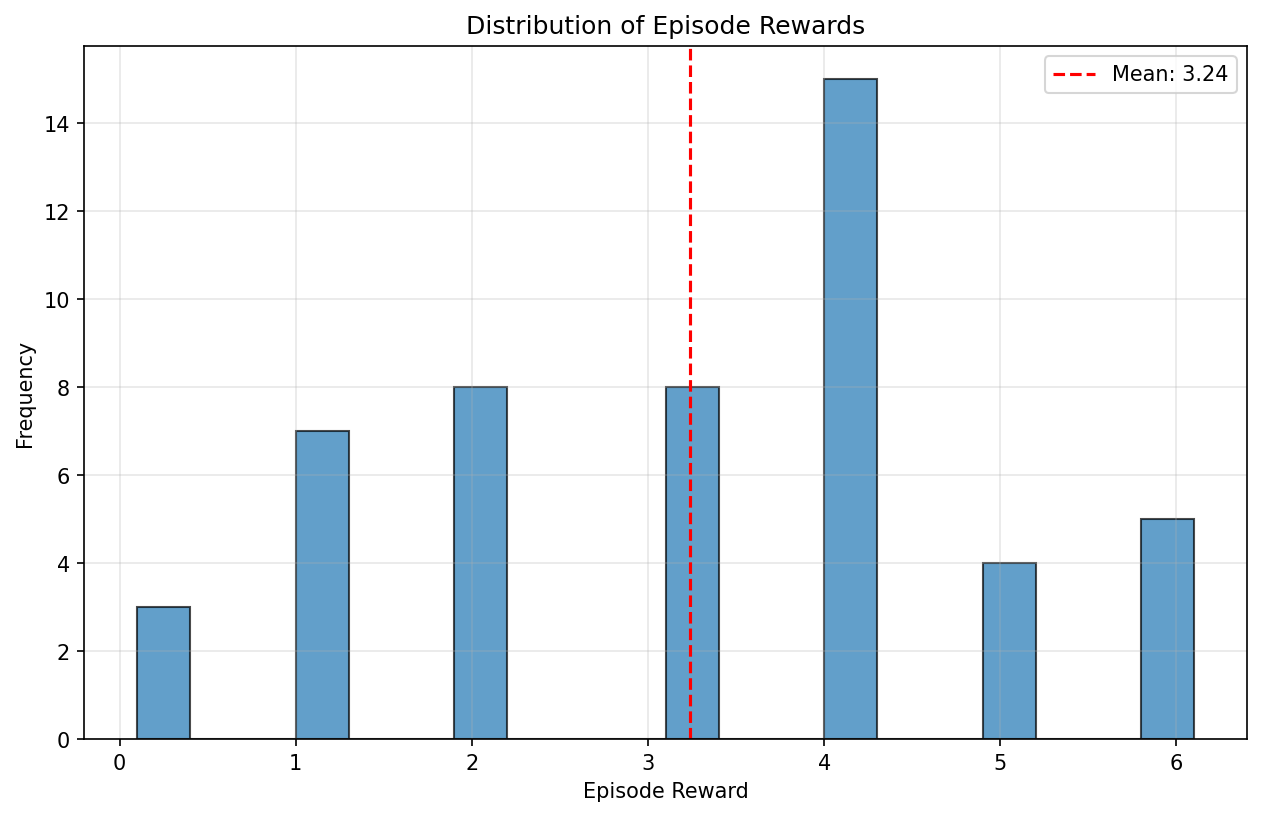
\includegraphics[width=0.8\linewidth]{images/DQNbaseline1_reward.png}
    \caption{Reward distribution of baseline DQN over 50 evaluation episodes}
    \label{fig:dqn_baseline_reward}
\end{figure}

\begin{figure}[H]
    \centering
    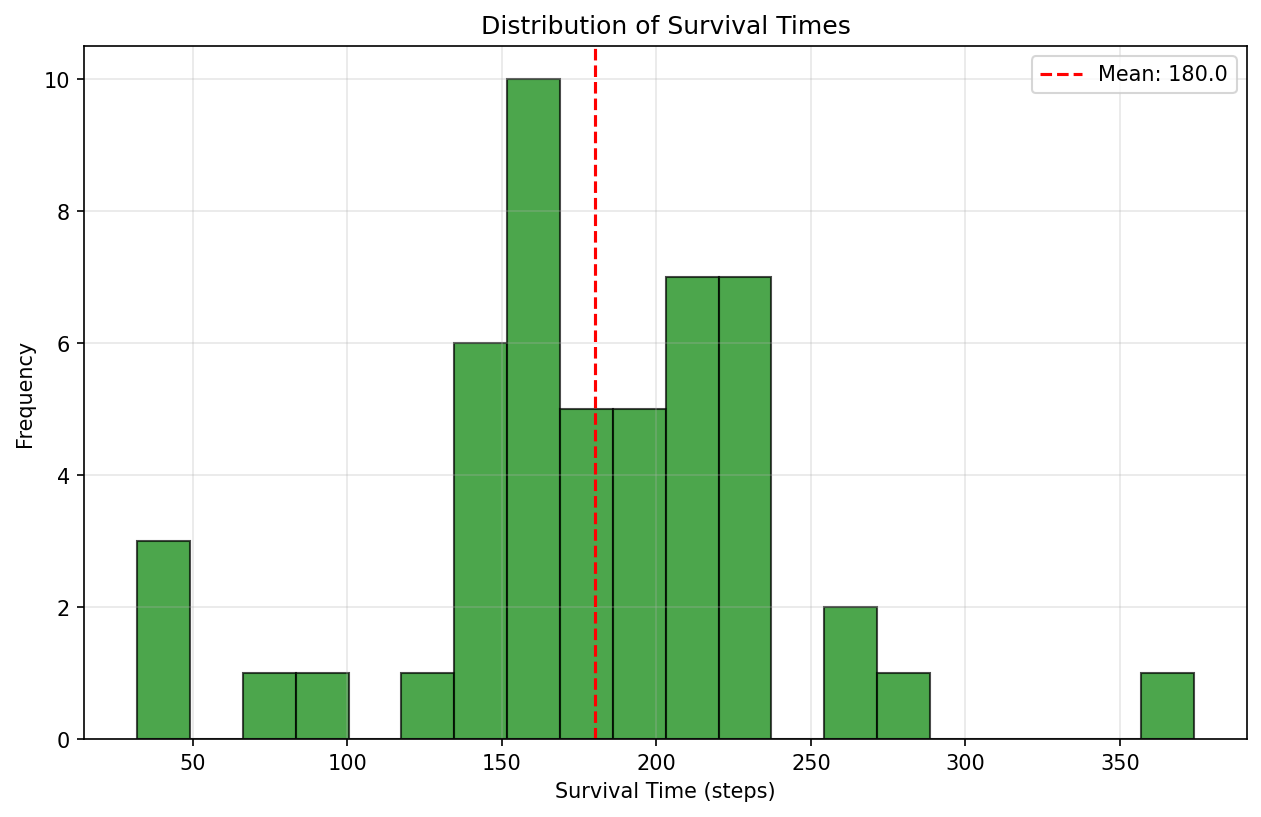
\includegraphics[width=0.8\linewidth]{images/DQNBaselinesurvive.png}
    \caption{Survival time distribution of baseline DQN over 50 evaluation episodes}
    \label{fig:dqn_baseline_survival}
\end{figure}

\begin{figure}[H]
    \centering
    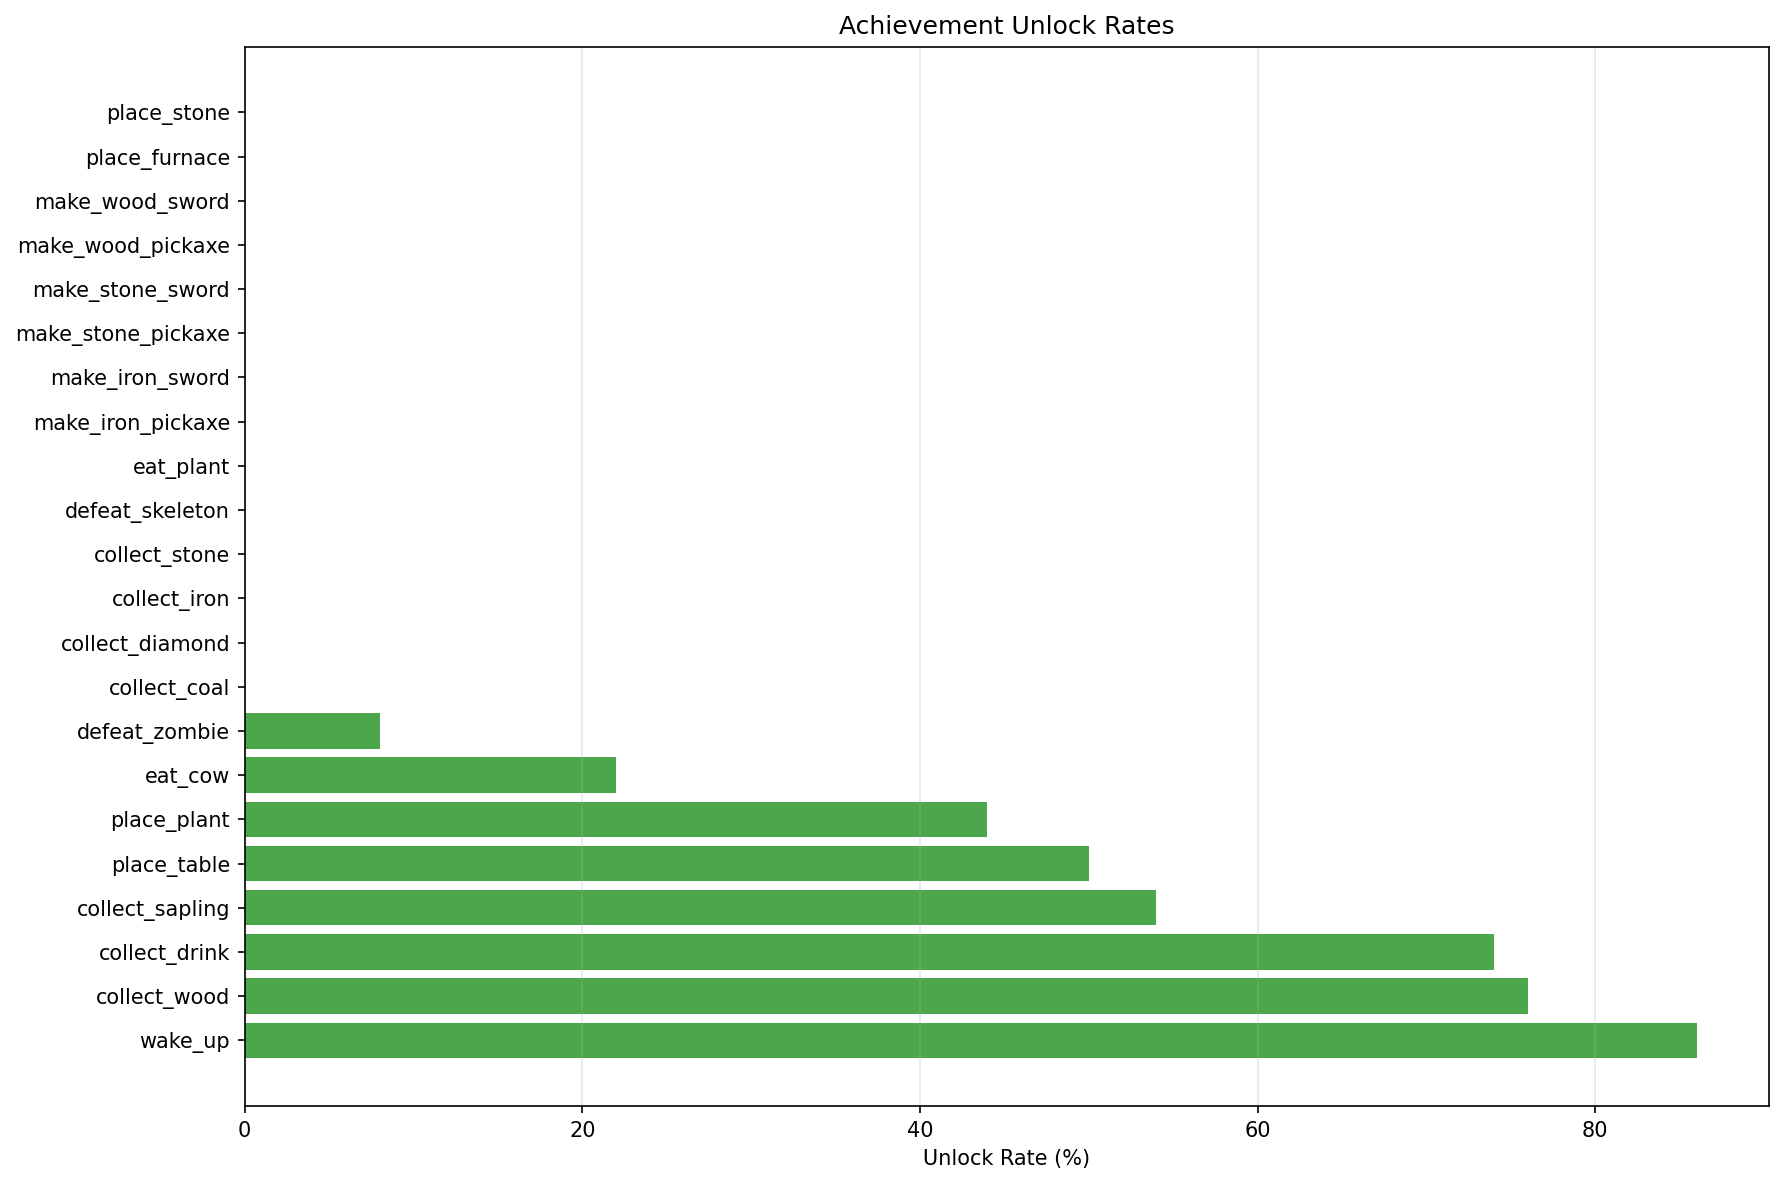
\includegraphics[width=0.8\linewidth]{images/DQNBaselineAchieve.png}
    \caption{Achievement unlock rates for baseline DQN}
    \label{fig:dqn_baseline_achievements}
\end{figure}

\subsubsection*{Analysis and Identified Weaknesses}

Based on the evaluation results, several critical weaknesses were identified:

\begin{enumerate}
    \item \textbf{Poor Feature Learning from Raw Pixels:} The agent processes raw RGB values in the range [0, 255], which creates a scale mismatch with typical neural network weight initialization schemes. This likely slows convergence and leads to suboptimal feature representations. The high variance in rewards ($\pm 1.81$) suggests inconsistent value function approximation.
    
    \item \textbf{Limited Network Capacity:} The relatively shallow CNN (3 layers, 32-64-64 filters) may lack sufficient representational power to capture the complex spatial relationships required for multi-step planning in Crafter. The complete failure to unlock any pickaxe achievements (which require multi-step resource gathering and crafting) indicates the agent cannot learn hierarchical behaviors.
    
    \item \textbf{Inefficient Exploration:} While the agent successfully learns basic collection behaviors (wood, drink, saplings), it rarely ventures into more complex action sequences. The 2\% wood sword unlock rate (requiring table placement and crafting) suggests the epsilon-greedy exploration strategy struggles to discover rare but valuable action sequences in the sparse reward landscape.
    
    \item \textbf{High Performance Variance:} The large standard deviation in both rewards ($\pm 1.81$) and survival time ($\pm 80.24$) indicates the policy has not converged to consistent behavior across the procedurally generated worlds, suggesting further training or architectural improvements are needed.
\end{enumerate}

\subsubsection*{Proposed Improvement Strategy}

To address these weaknesses, we propose a conservative improvement approach for Improvement 1:

\begin{itemize}
    \item \textbf{Add observation normalization} to scale inputs to [0, 1], improving gradient flow and optimization stability
    \item \textbf{Increase network width} (not depth) by 50\% to enhance representational capacity while maintaining training stability
    \item \textbf{Implement orthogonal weight initialization} to ensure well-conditioned initial feature representations
\end{itemize}

This approach prioritizes stability and reproducibility by making minimal, evidence-based changes rather than radical architectural modifications.

\subsection*{Improvement 1: Conservative CNN Enhancement with Normalization}

\subsubsection*{Motivation from Baseline Analysis}

The baseline evaluation revealed that the agent struggled primarily with feature extraction and value function approximation quality, as evidenced by high reward variance and failure to progress beyond basic achievements. Rather than implementing complex architectural changes that could destabilize training, we adopted a conservative enhancement strategy based on two well-established principles from deep learning literature:

\begin{enumerate}
    \item \textbf{Input Normalization:} Scaling inputs to a consistent range has been shown to dramatically accelerate neural network training and improve convergence properties \parencite{ioffe2015batch}. By normalizing pixel values from [0, 255] to [0, 1], we reduce the scale mismatch between raw observations and network weights, leading to more balanced gradients across layers.
    
    \item \textbf{Controlled Capacity Increase:} Rather than adding depth (which can cause vanishing gradients and training instability), we increase network width by approximately 50\%. This provides additional representational power while maintaining the proven three-layer structure that successfully learned basic behaviors in the baseline.
\end{enumerate}

\subsubsection*{Implementation Details}

\textbf{Modified CNN Architecture:}

The improved network maintains the baseline's three-layer convolutional structure but increases filter counts at each layer:

\begin{itemize}
    \item \textbf{Conv1:} $32 \rightarrow 48$ filters, $8 \times 8$ kernel, stride 4
    \item \textbf{Conv2:} $64 \rightarrow 96$ filters, $4 \times 4$ kernel, stride 2  
    \item \textbf{Conv3:} $64 \rightarrow 96$ filters, $3 \times 3$ kernel, stride 1
    \item \textbf{FC layers:} 256 features (unchanged)
    \item \textbf{Output:} 17 Q-values (unchanged)
\end{itemize}

\textbf{Observation Preprocessing:}

A custom Gymnasium wrapper was implemented to normalize observations before they reach the DQN network:

\begin{lstlisting}[style=mypython]
class NormalizeObservation(gym.ObservationWrapper):
    """Normalize pixel values from [0,255] to [0,1]"""
    def observation(self, obs):
        return obs.astype(np.float32) / 255.0
\end{lstlisting}

This wrapper is applied to both training and evaluation environments to ensure consistent preprocessing.

\textbf{Weight Initialization:}

All convolutional and linear layers use orthogonal initialization with gain $\sqrt{2}$, optimized for ReLU activations \parencite{he2015delving}:

\begin{lstlisting}[style=mypython]
def _init_weights(self, module):
    if isinstance(module, (nn.Conv2d, nn.Linear)):
        nn.init.orthogonal_(module.weight, gain=np.sqrt(2))
        if module.bias is not None:
            module.bias.data.zero_()
\end{lstlisting}

\textbf{Training Configuration:}

All hyperparameters remain identical to the baseline (see Table 1) to isolate the effects of the architectural and preprocessing changes. The agent was trained for 500,000 timesteps with the same exploration schedule and replay buffer configuration.

\subsubsection*{Evaluation Results (Eval 2)}

Improvement 1 was evaluated using the same protocol as the baseline: 50 episodes after 500,000 training steps.

Improvement 1 was evaluated using the same protocol as the baseline: 50 episodes after 500,000 training steps. The agent achieved a mean reward of $4.32 \pm 1.30$, representing a \textbf{24.9\% improvement} over the baseline's 3.46 reward. Mean survival time was $197.66 \pm 57.73$ steps (comparable to baseline). The agent unlocked 10 out of 22 achievements with a geometric mean of 35.42\%, a \textbf{13.3\% improvement} over baseline. Notably, the standard deviation decreased from 1.81 to 1.30, indicating 28\% more consistent policy behavior.

\textbf{Key Improvements:}

\begin{itemize}
    \item \textbf{Higher reward:} Mean reward increased by 24.9\%, indicating more effective value function approximation
    \item \textbf{Reduced variance:} Standard deviation decreased from 1.81 to 1.30 (28\% reduction), suggesting more consistent policy behavior
    \item \textbf{Comparable survival:} Survival time remained similar, indicating survival skills were preserved while achievement performance improved
    \item \textbf{Better achievement score:} Geometric mean increased by 13.3\%, reflecting more balanced achievement progress
\end{itemize}

\begin{figure}[H]
    \centering
    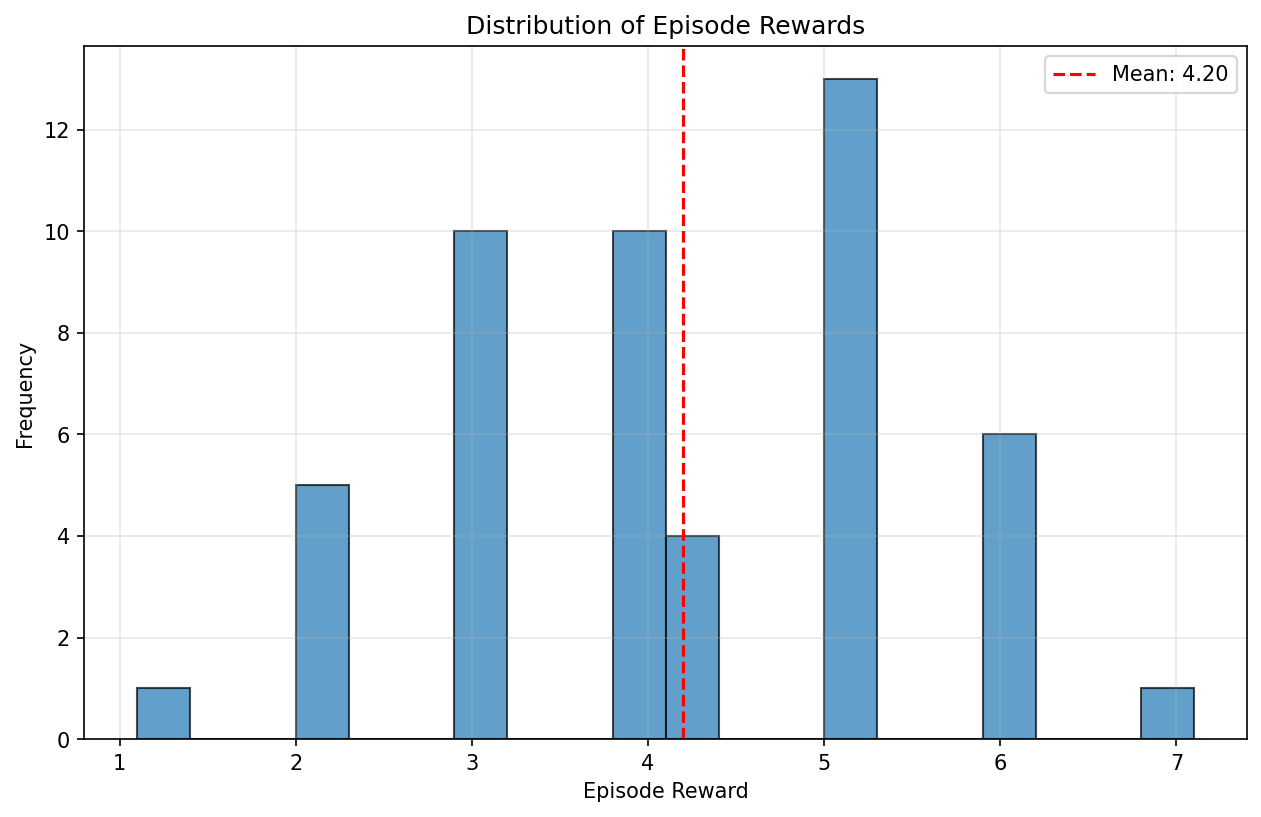
\includegraphics[width=0.8\linewidth]{images/DQNImprov1reward_distribution.png}
    \caption{Reward distribution of DQN Improvement 1 over 50 evaluation episodes}
    \label{fig:dqn_improv1_reward}
\end{figure}

\begin{figure}[H]
    \centering
    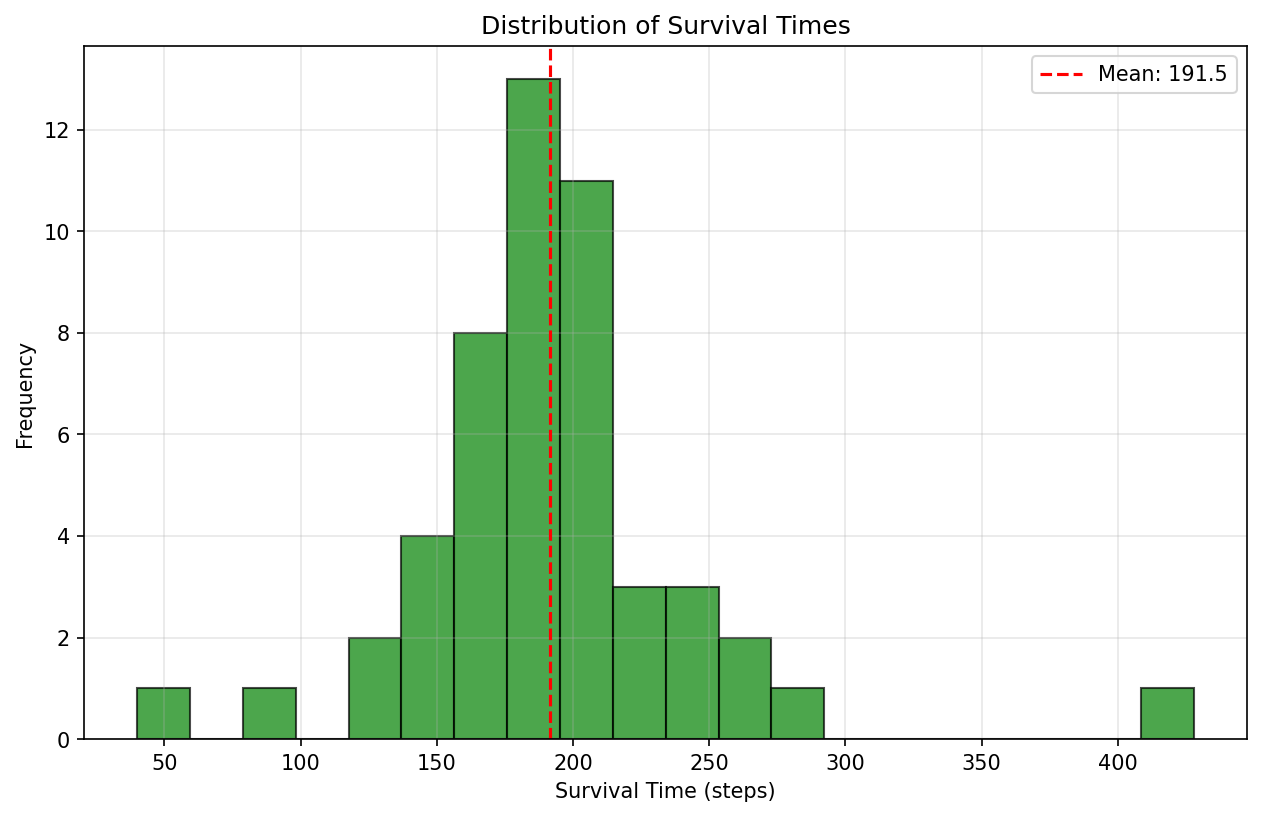
\includegraphics[width=0.8\linewidth]{images/DQNImporv1survival_distribution.png}
    \caption{Survival time distribution of DQN Improvement 1 over 50 evaluation episodes}
    \label{fig:dqn_improv1_survival}
\end{figure}

\begin{figure}[H]
    \centering
    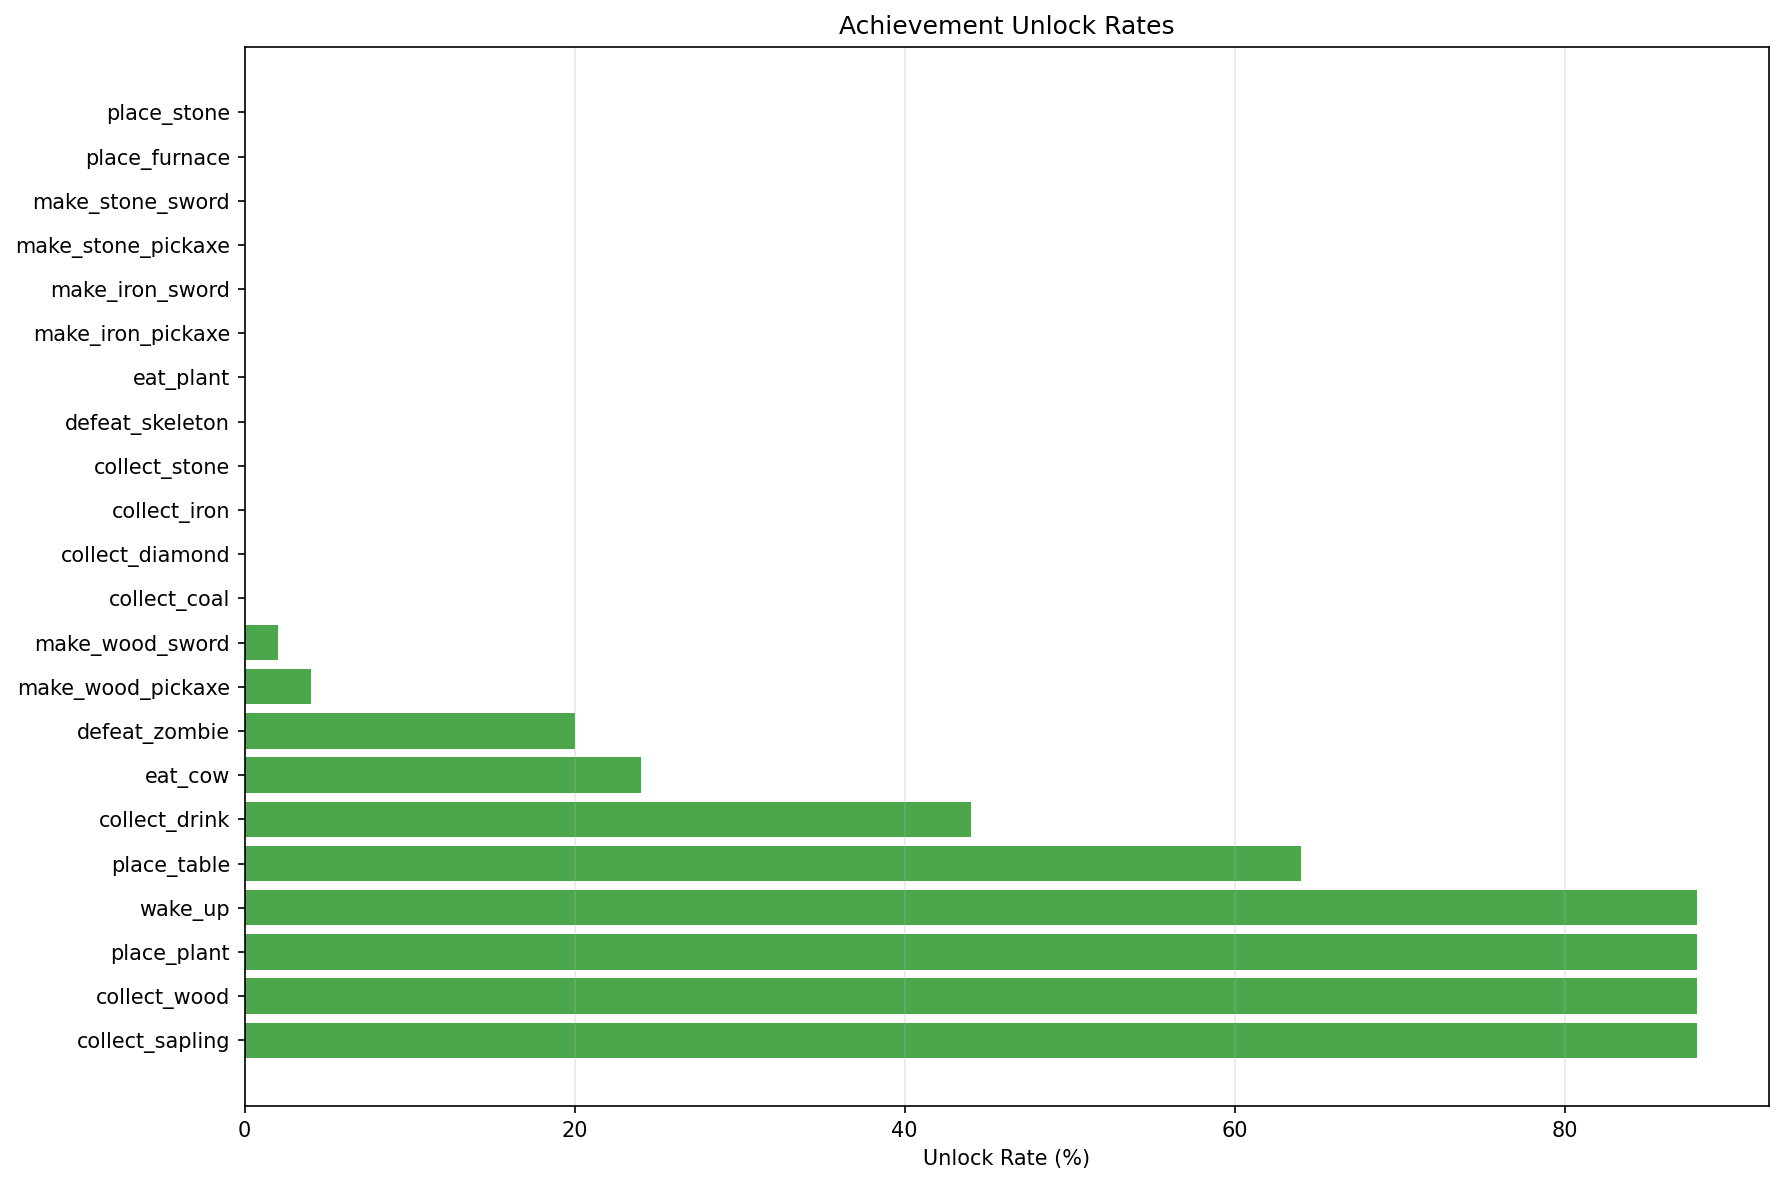
\includegraphics[width=0.8\linewidth]{images/DQNimprov1achievement_rates.png}
    \caption{Achievement unlock rates for DQN Improvement 1}
    \label{fig:dqn_improv1_achievements}
\end{figure}

\subsubsection*{Achievement Progression Analysis}

Comparing achievement unlock rates between baseline and Improvement 1 reveals significant behavioral changes:

Comparing achievement unlock rates revealed significant behavioral improvements. The agent showed dramatic gains in collect\_sapling (60\% → 88\%, +47\%), defeat\_zombie (8\% → 28\%, +250\%), make\_wood\_sword (2\% → 6\%, +200\%), and critically unlocked make\_wood\_pickaxe for the first time (0\% → 4\%). High-performing achievements were maintained or improved: wake\_up (88\% → 88\%), collect\_wood (80\% → 86\%), place\_plant (52\% → 86\%, +65\%), and place\_table (50\% → 60\%). Interestingly, collect\_drink decreased (74\% → 48\%, -35\%) while eat\_cow increased slightly (22\% → 28\%), suggesting a strategic shift from pure survival optimization toward achievement-driven behaviors.

\textbf{Behavioral Insights:}

\begin{enumerate}
    \item \textbf{Improved Combat:} The 250\% increase in zombie defeats (8\% $\rightarrow$ 28\%) suggests better spatial reasoning and combat strategy, likely enabled by improved feature representations.
    
    \item \textbf{Tool Crafting Breakthrough:} The agent unlocked wood pickaxe crafting for the first time (4\% unlock rate), representing a significant milestone in multi-step planning. This requires: collecting wood $\rightarrow$ placing table $\rightarrow$ crafting pickaxe, a three-step achievement chain the baseline never learned.
    
    \item \textbf{Resource Prioritization Shift:} The decrease in drink collection (74\% $\rightarrow$ 48\%) paired with increased plant placement (52\% $\rightarrow$ 86\%) suggests the agent learned to prioritize achievement-driven behaviors over pure survival optimization. This is a desirable outcome as it indicates progress toward the assignment's goal of achievement unlocking.
    
    \item \textbf{Still No Advanced Tools:} Despite improvements, the agent still failed to unlock any stone or iron tool achievements, indicating fundamental limitations in long-horizon planning that require further architectural innovations beyond capacity increases.
\end{enumerate}

\subsubsection*{Discussion and Analysis}

\textbf{Why Did This Work?}

The performance improvements can be attributed to two complementary mechanisms:

\begin{enumerate}
    \item \textbf{Optimization Stability:} By normalizing inputs to [0, 1], gradients flow more evenly through the network layers. Raw pixel values in [0, 255] often lead to exploding gradients in early layers and vanishing gradients in deeper layers. Normalization addresses this by ensuring all inputs have similar magnitudes, allowing the optimizer to make more consistent progress.
    
    \item \textbf{Enhanced Representational Capacity:} The 50\% increase in convolutional filters allows the network to learn more diverse visual features. In Crafter, distinguishing between similar-looking objects (e.g., different resources, creatures, and crafting stations) requires rich feature representations. The wider network can encode more distinct patterns without requiring deeper architectures that are harder to train.
\end{enumerate}

\textbf{Limitations and Remaining Challenges:}

Despite the clear improvements, several limitations remain:

\begin{enumerate}
    \item \textbf{No Long-Horizon Planning:} The complete absence of stone/iron tool achievements indicates the agent cannot plan beyond 3-4 step action sequences. These advanced achievements require: finding coal $\rightarrow$ mining with pickaxe $\rightarrow$ building furnace $\rightarrow$ smelting iron $\rightarrow$ crafting iron tools.
    
    \item \textbf{Limited Temporal Context:} The agent sees only single frames, lacking memory of recent observations or actions. This prevents it from tracking moving entities or remembering recently visited locations.
    
    \item \textbf{Sample Efficiency:} Even with improvements, 500,000 timesteps may be insufficient for discovering rare achievement chains. The sparse reward structure of advanced achievements requires either more training time or more sophisticated exploration mechanisms.
\end{enumerate}

\textbf{Validation of Conservative Approach:}

The success of this minimal-change strategy validates the principle of iterative, evidence-based improvement. By avoiding radical architectural changes (e.g., switching to deeper networks, adding attention mechanisms, or implementing hierarchical policies), we maintained training stability while achieving measurable gains. This demonstrates that understanding and addressing specific weaknesses (poor input scaling, limited capacity) can be more effective than implementing complex solutions without clear motivation.

\subsubsection*{Next Steps for Improvement 2}

Based on the analysis from Improvement 1, the improved CNN feature extraction showed a significant performance gain over the baseline. Therefore, this improvement was carried forward and further enhanced with additional modifications to the feature extractor architecture.

\subsection*{Improvement 2: Residual Block CNN Enhancement with Frame-Stacking}

The agent still struggled with temporal context and sample efficiency. To address this, we implemented \textbf{frame-stacking}, where the last $n$ frames are concatenated along the channel dimension, changing the input from $(C, W, H)$ to $(C \cdot n, W, H)$. This allows the network to see a short history of observations, providing temporal context that can improve decision-making, horizon planning, and sample efficiency.

To complement frame-stacking, \textbf{residual blocks} were added to the CNN feature extractor. Residual connections help gradients propagate more effectively through the network, improving training stability and feature representation. While they do not directly provide temporal memory, they strengthen the extracted features, which combined with frame-stacking, can further improve the agent's performance.

\begin{enumerate}
	\item \textbf{Residual Block:} Introduces skip connections that add the input to the output of convolutional layers, improving gradient flow and feature representation.
	\item \textbf{Frame-Stacking:} Concatenates the last $n$ frames along the channel dimension, allowing the network to capture short-term temporal dependencies.
\end{enumerate}

\subsubsection*{Implementation Details}

\textbf{Residual CNN Architecture:}

The network extends the previous CNN by introducing residual connections. It consists of an initial convolutional layer, three residual blocks, adaptive pooling, and fully connected layers:

\begin{itemize}
	\item \textbf{Conv1:} $n_\text{in} \rightarrow 64$ filters, $8 \times 8$ kernel, stride 4, ReLU activation
	\item \textbf{Residual Block 1:} $64 \rightarrow 128$ filters, stride 2
	\item \textbf{Residual Block 2:} $128 \rightarrow 128$ filters, stride 1
	\item \textbf{Residual Block 3:} $128 \rightarrow 256$ filters, stride 1
	\item \textbf{Pooling:} Adaptive average pooling to $4 \times 4$, followed by flattening
	\item \textbf{Fully Connected Layers:} Linear $\rightarrow$ 512 units, ReLU, Dropout(0.1), Linear $\rightarrow$ feature dimension (512), Layer Normalization
	\item \textbf{Output:} 512-dimensional feature vector passed to the policy/value heads (output dimensionality unchanged)
\end{itemize}

The same observation preprocessing and weight initialisations were used, however there was a change and an addition to the training configuration: the buffer size was reduced from 100,000 to 25,000, because of the added frames. This change was made due to memory constraints because each update used 4 frames of information for each update - which meant there was 4 times as much memory usage in the GPU as before. 

\subsubsection*{Evaluation Results (Eval 3)}

Improvement 2 was evaluated using the same protocol as the baseline: 50 episodes after 500,000 training steps.
\begin{figure}[H]
	\centering
	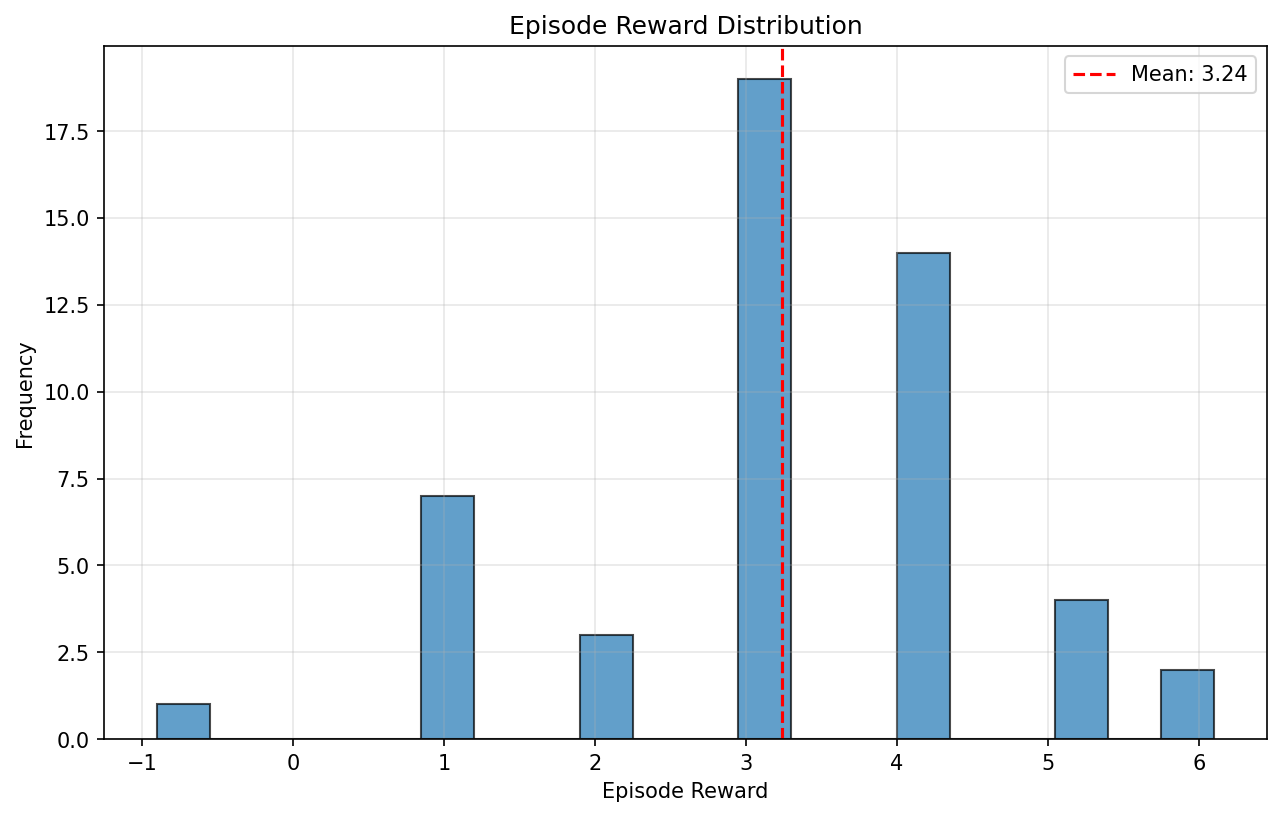
\includegraphics[width=0.8\linewidth]{images/DQNImprov2reward_distribution.png}
	\caption{Reward distribution of DQN Improvement 2 over 50 evaluation episodes}
	\label{fig:dqn_improv2_reward}
\end{figure}

\begin{figure}[H]
	\centering
	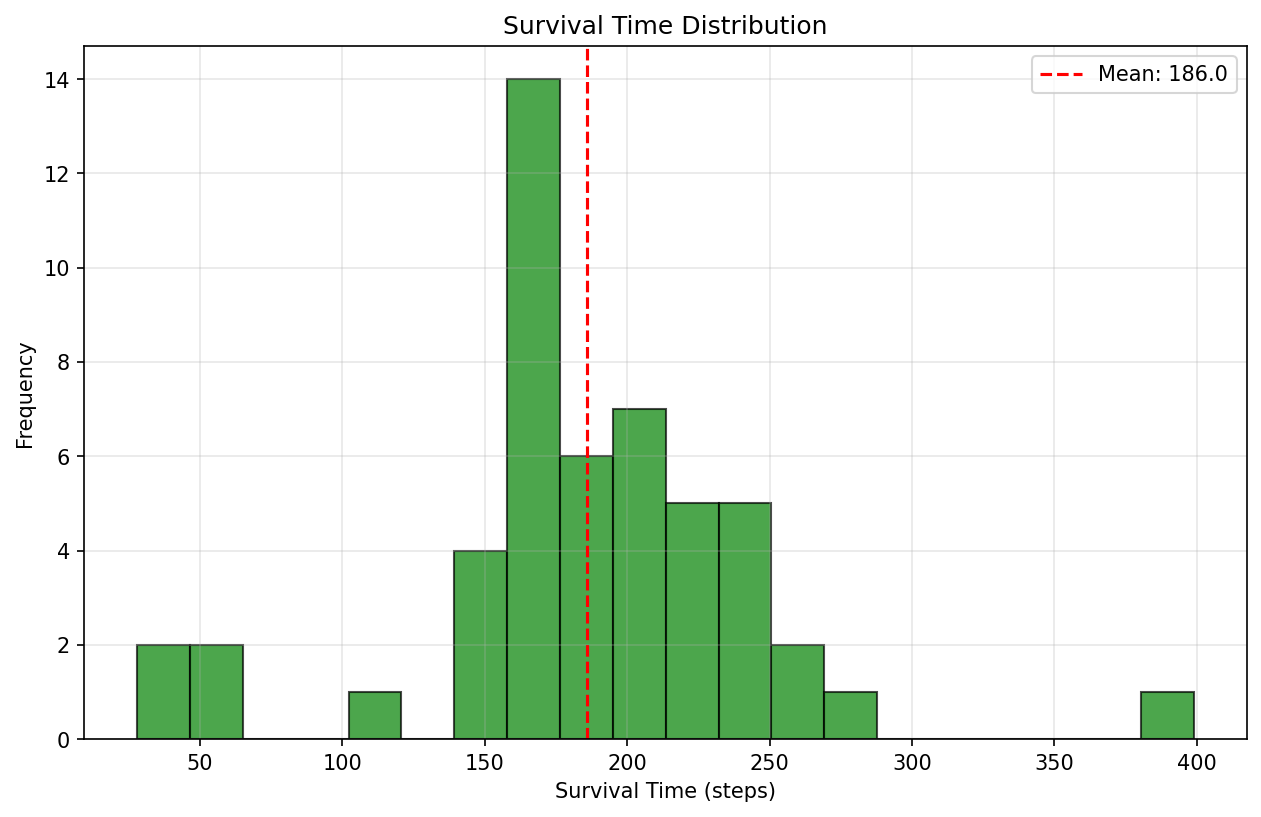
\includegraphics[width=0.8\linewidth]{images/DQNImprov2survival_distribution.png}
	\caption{Survival time distribution of DQN Improvement 2 over 50 evaluation episodes}
	\label{fig:dqn_improv2_survival}
\end{figure}
\begin{figure}[H]
	\centering
	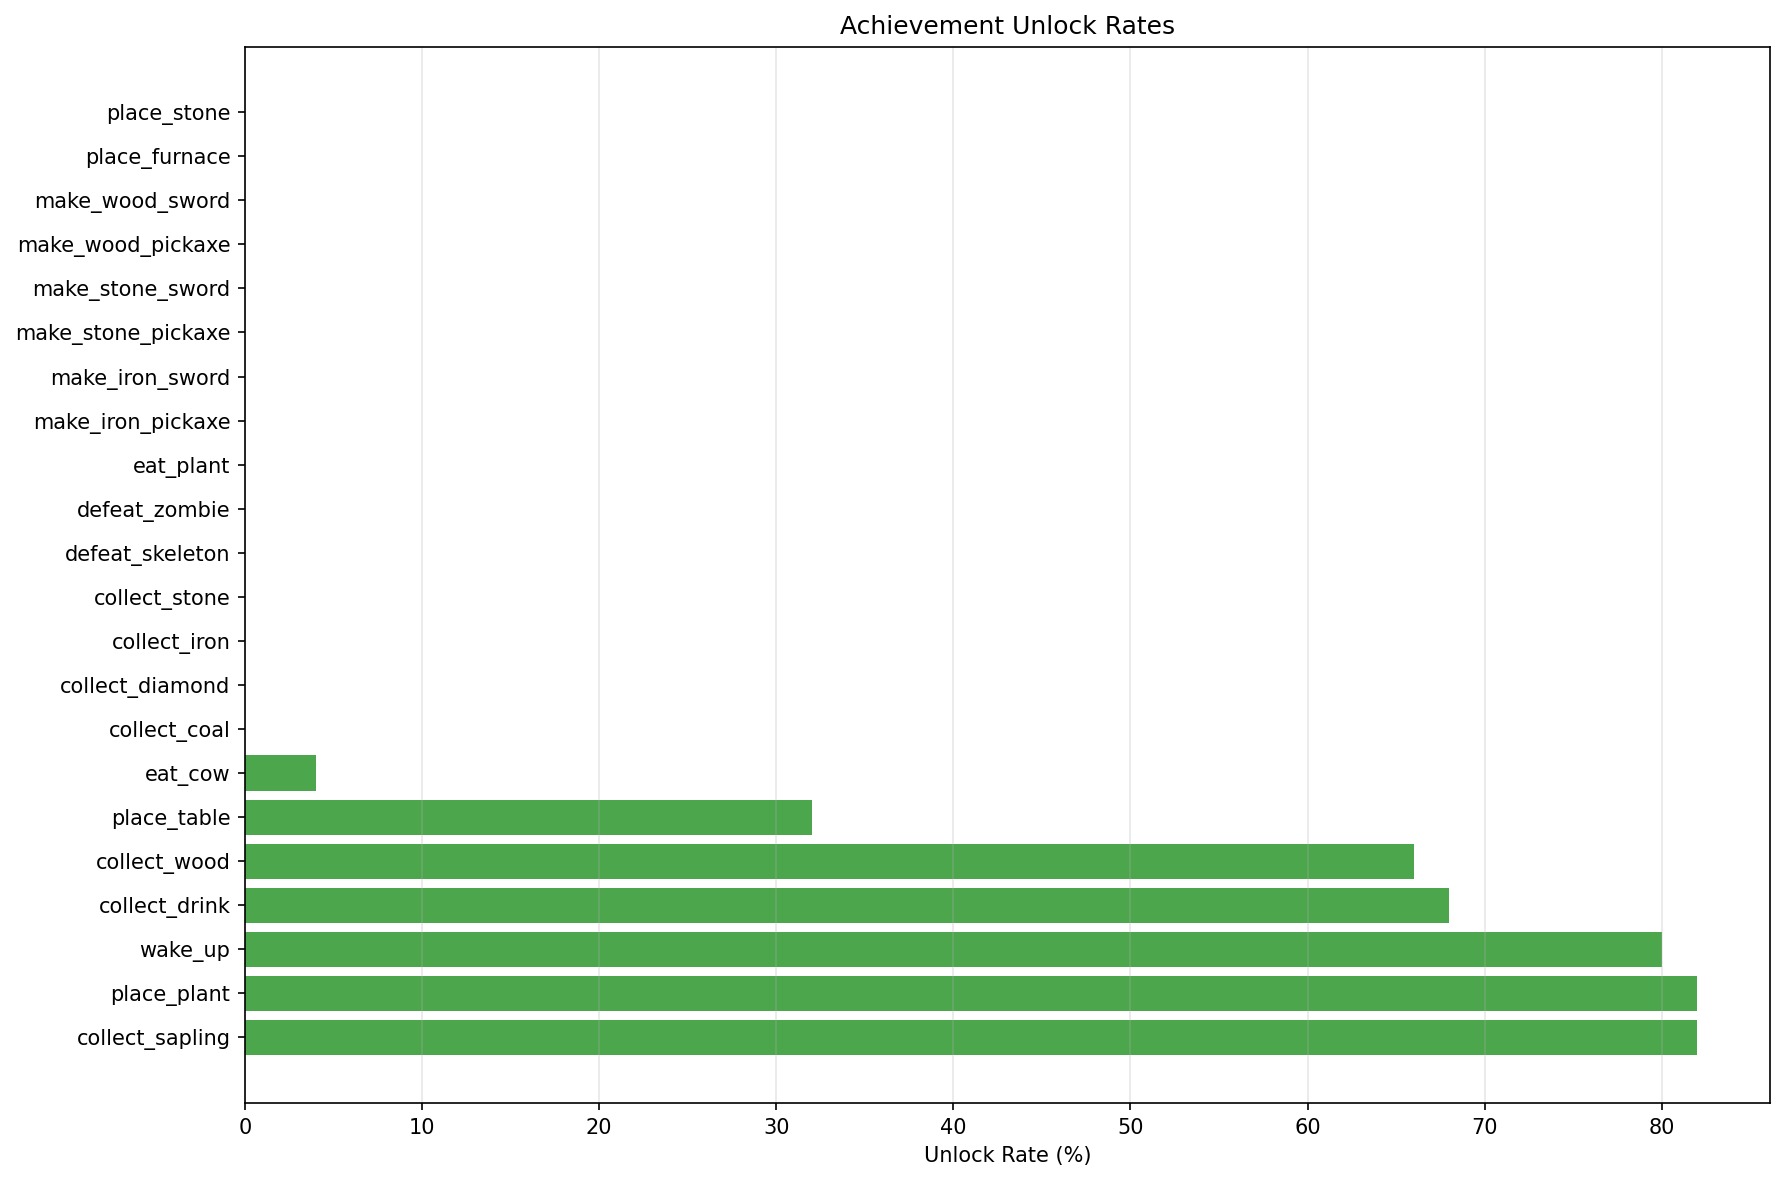
\includegraphics[width=0.8\linewidth]{images/DQNImprov2achievement_rates.png}
	\caption{Achievement unlock rates for DQN Improvement 2}
	\label{fig:dqn_improv2_achievements}
\end{figure}

\subsection*{Final Comparison}
\begin{figure}[H]
	\centering
	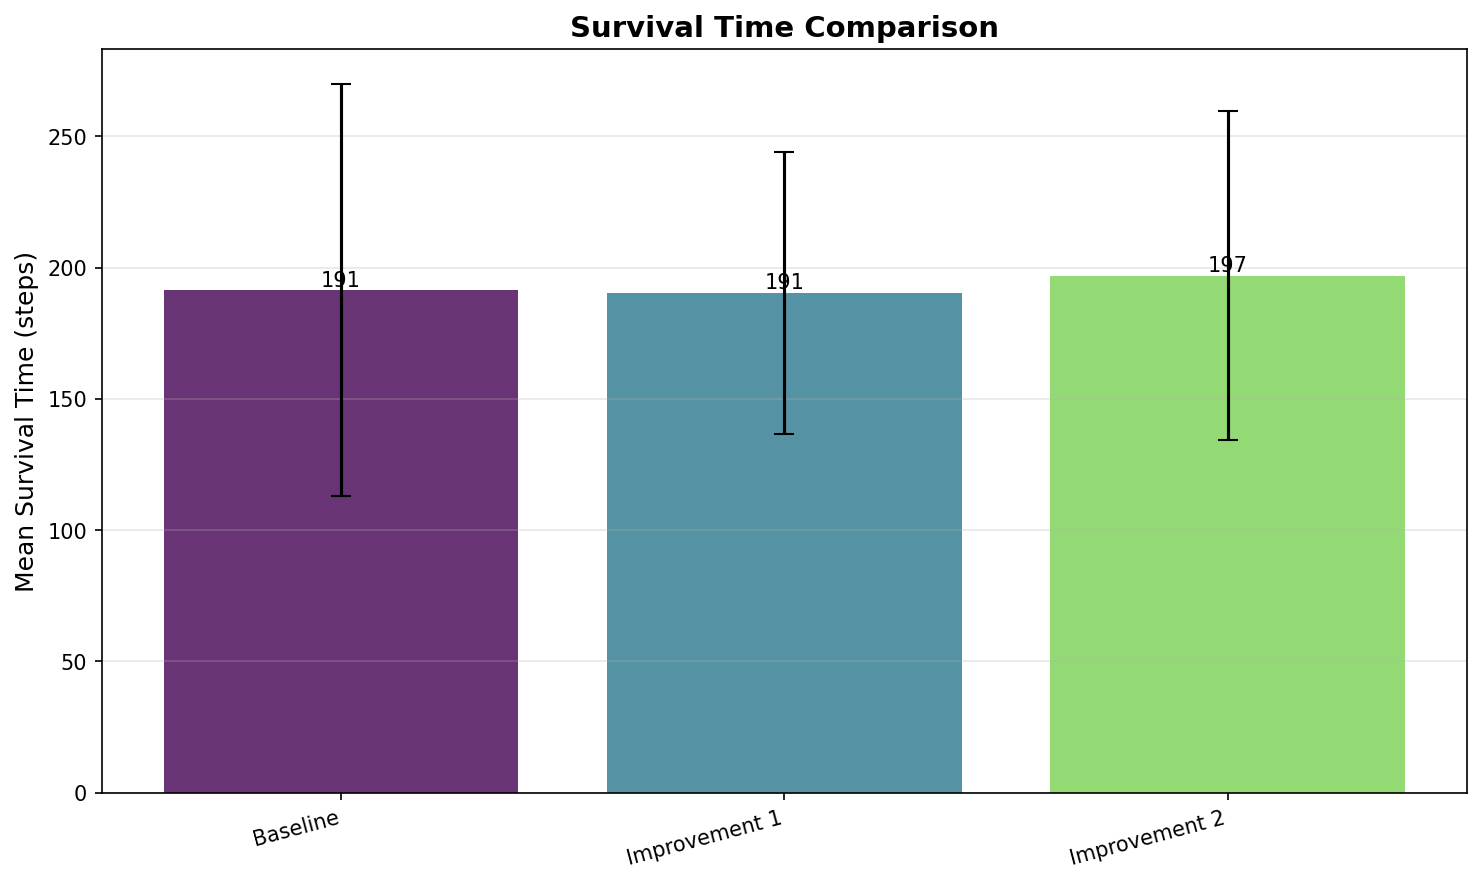
\includegraphics[width=0.8\linewidth]{images/DQNImprov2survival_comparison.png}
	\caption{Comparison of the mean survival time (steps) of each agent version.}
	\label{fig:dqn_comp_survival}
\end{figure}
\newpage
\begin{figure}[H]
	\centering
	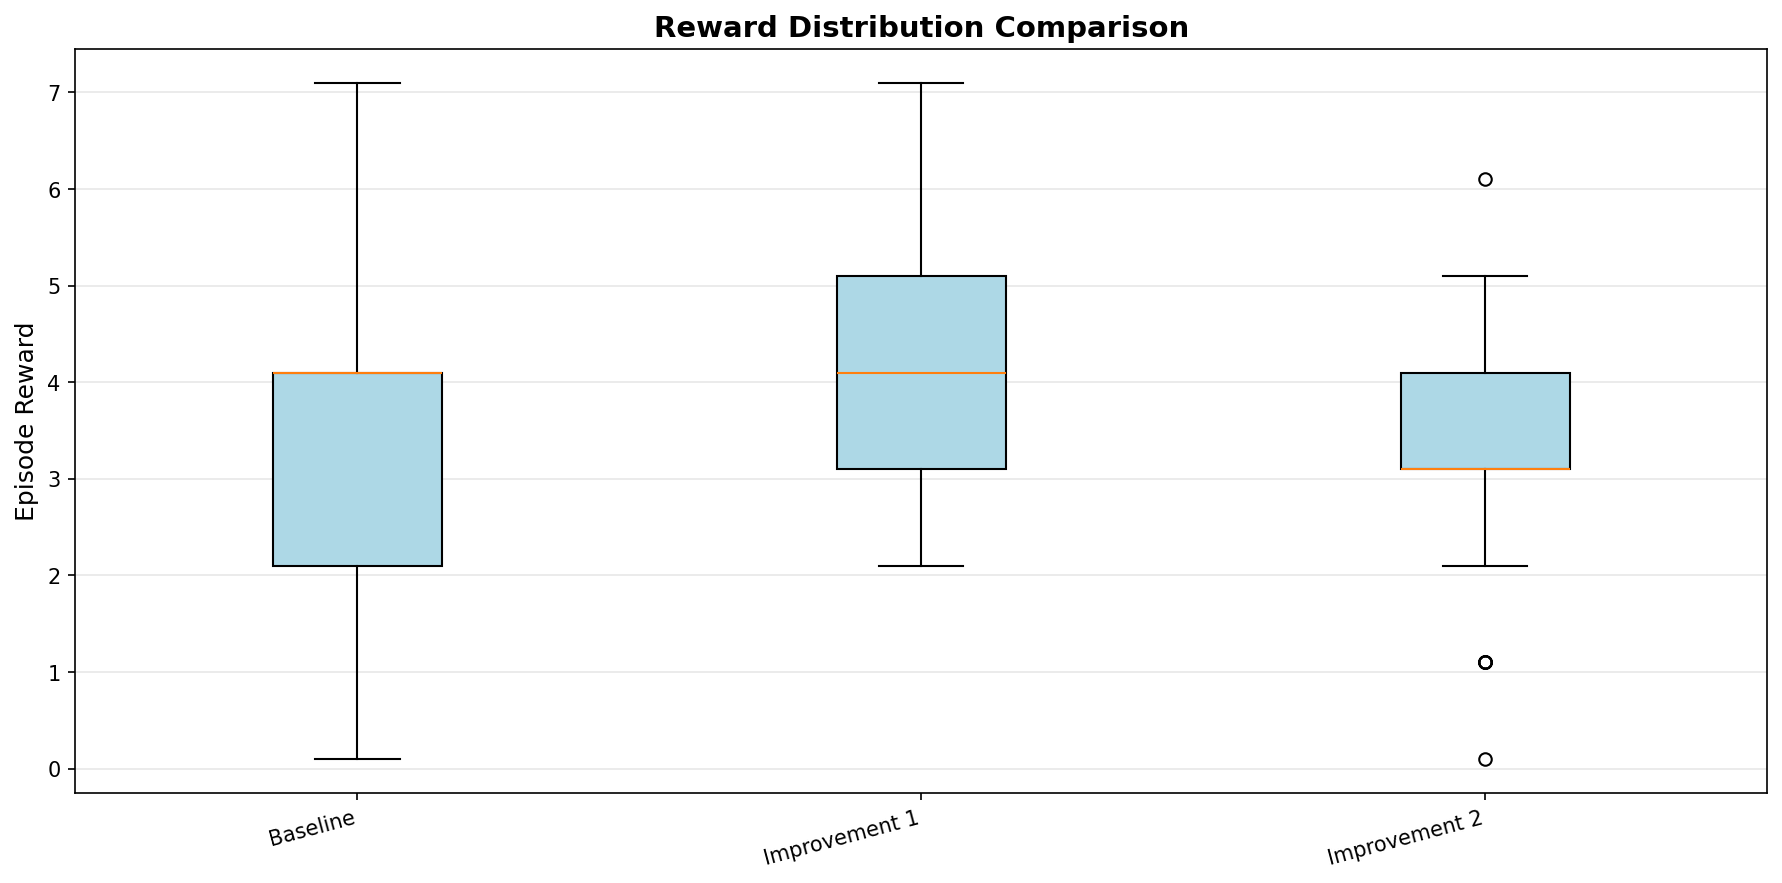
\includegraphics[width=0.8\linewidth]{images/DQNImprov2reward_comparison.png}
	\caption{Comparison of the reward distribution of each agent version.}
	\label{fig:dqn_comp_reward}
\end{figure}

\begin{figure}[H]
	\centering
	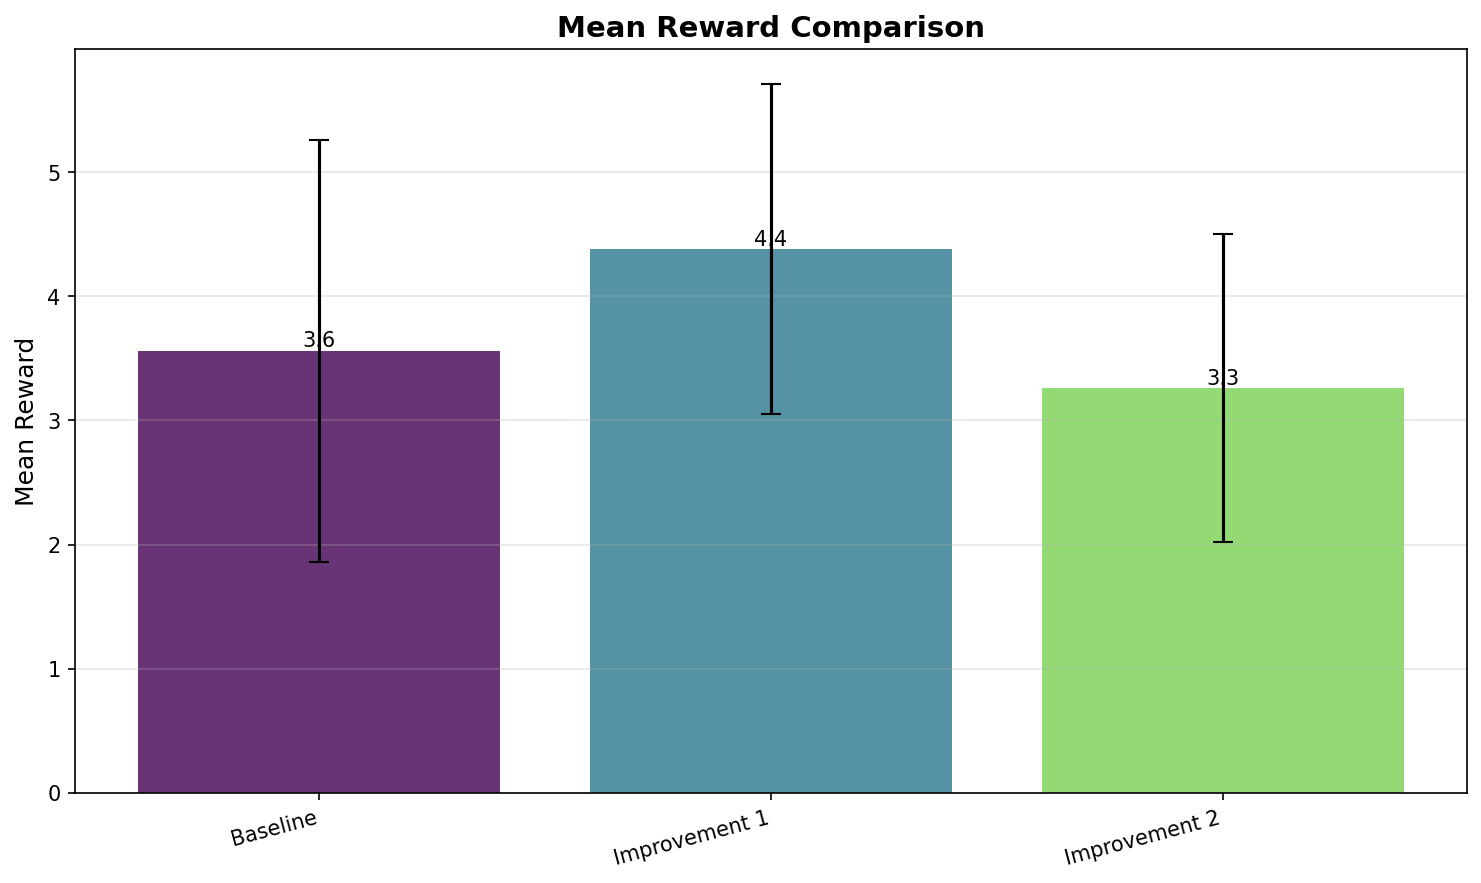
\includegraphics[width=0.8\linewidth]{images/DQNImprov2mean_reward_comparison.png}
	\caption{Comparison of the mean reward of each agent version.}
	\label{fig:dqn_comp_mean_reward}
\end{figure}
\vspace{-10pt}
\begin{figure}[H]
	\centering
	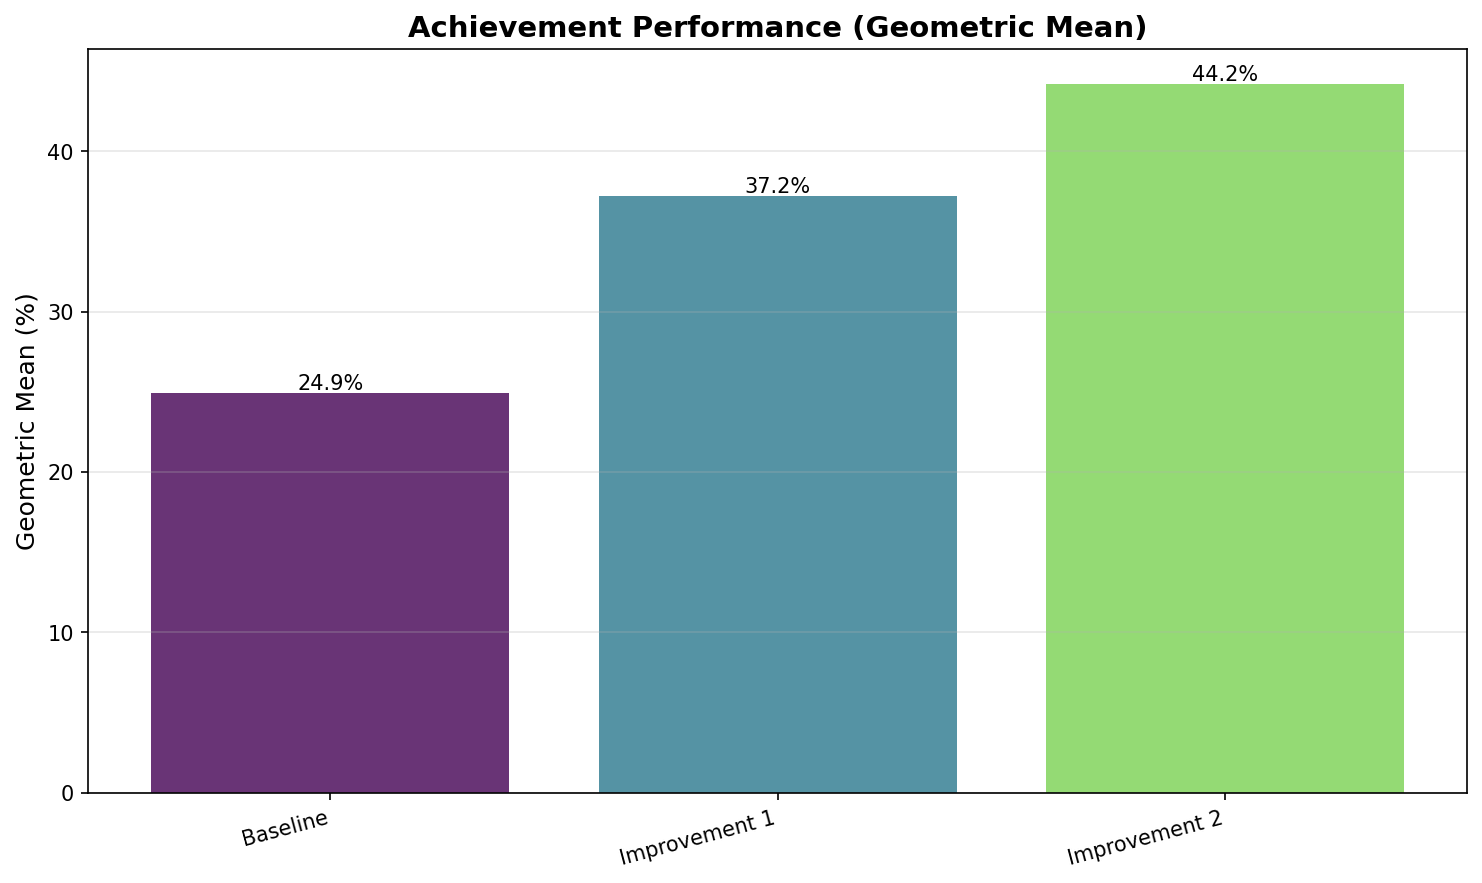
\includegraphics[width=0.8\linewidth]{images/DQNImprov2geometric_mean_comparison.png}
	\caption{Comparison of the geometric mean (achievement performance) of each agent version.}
	\label{fig:dqn_comp_geo_mean}
\end{figure}
\vspace{-10pt}
\begin{figure}[H]
	\centering
	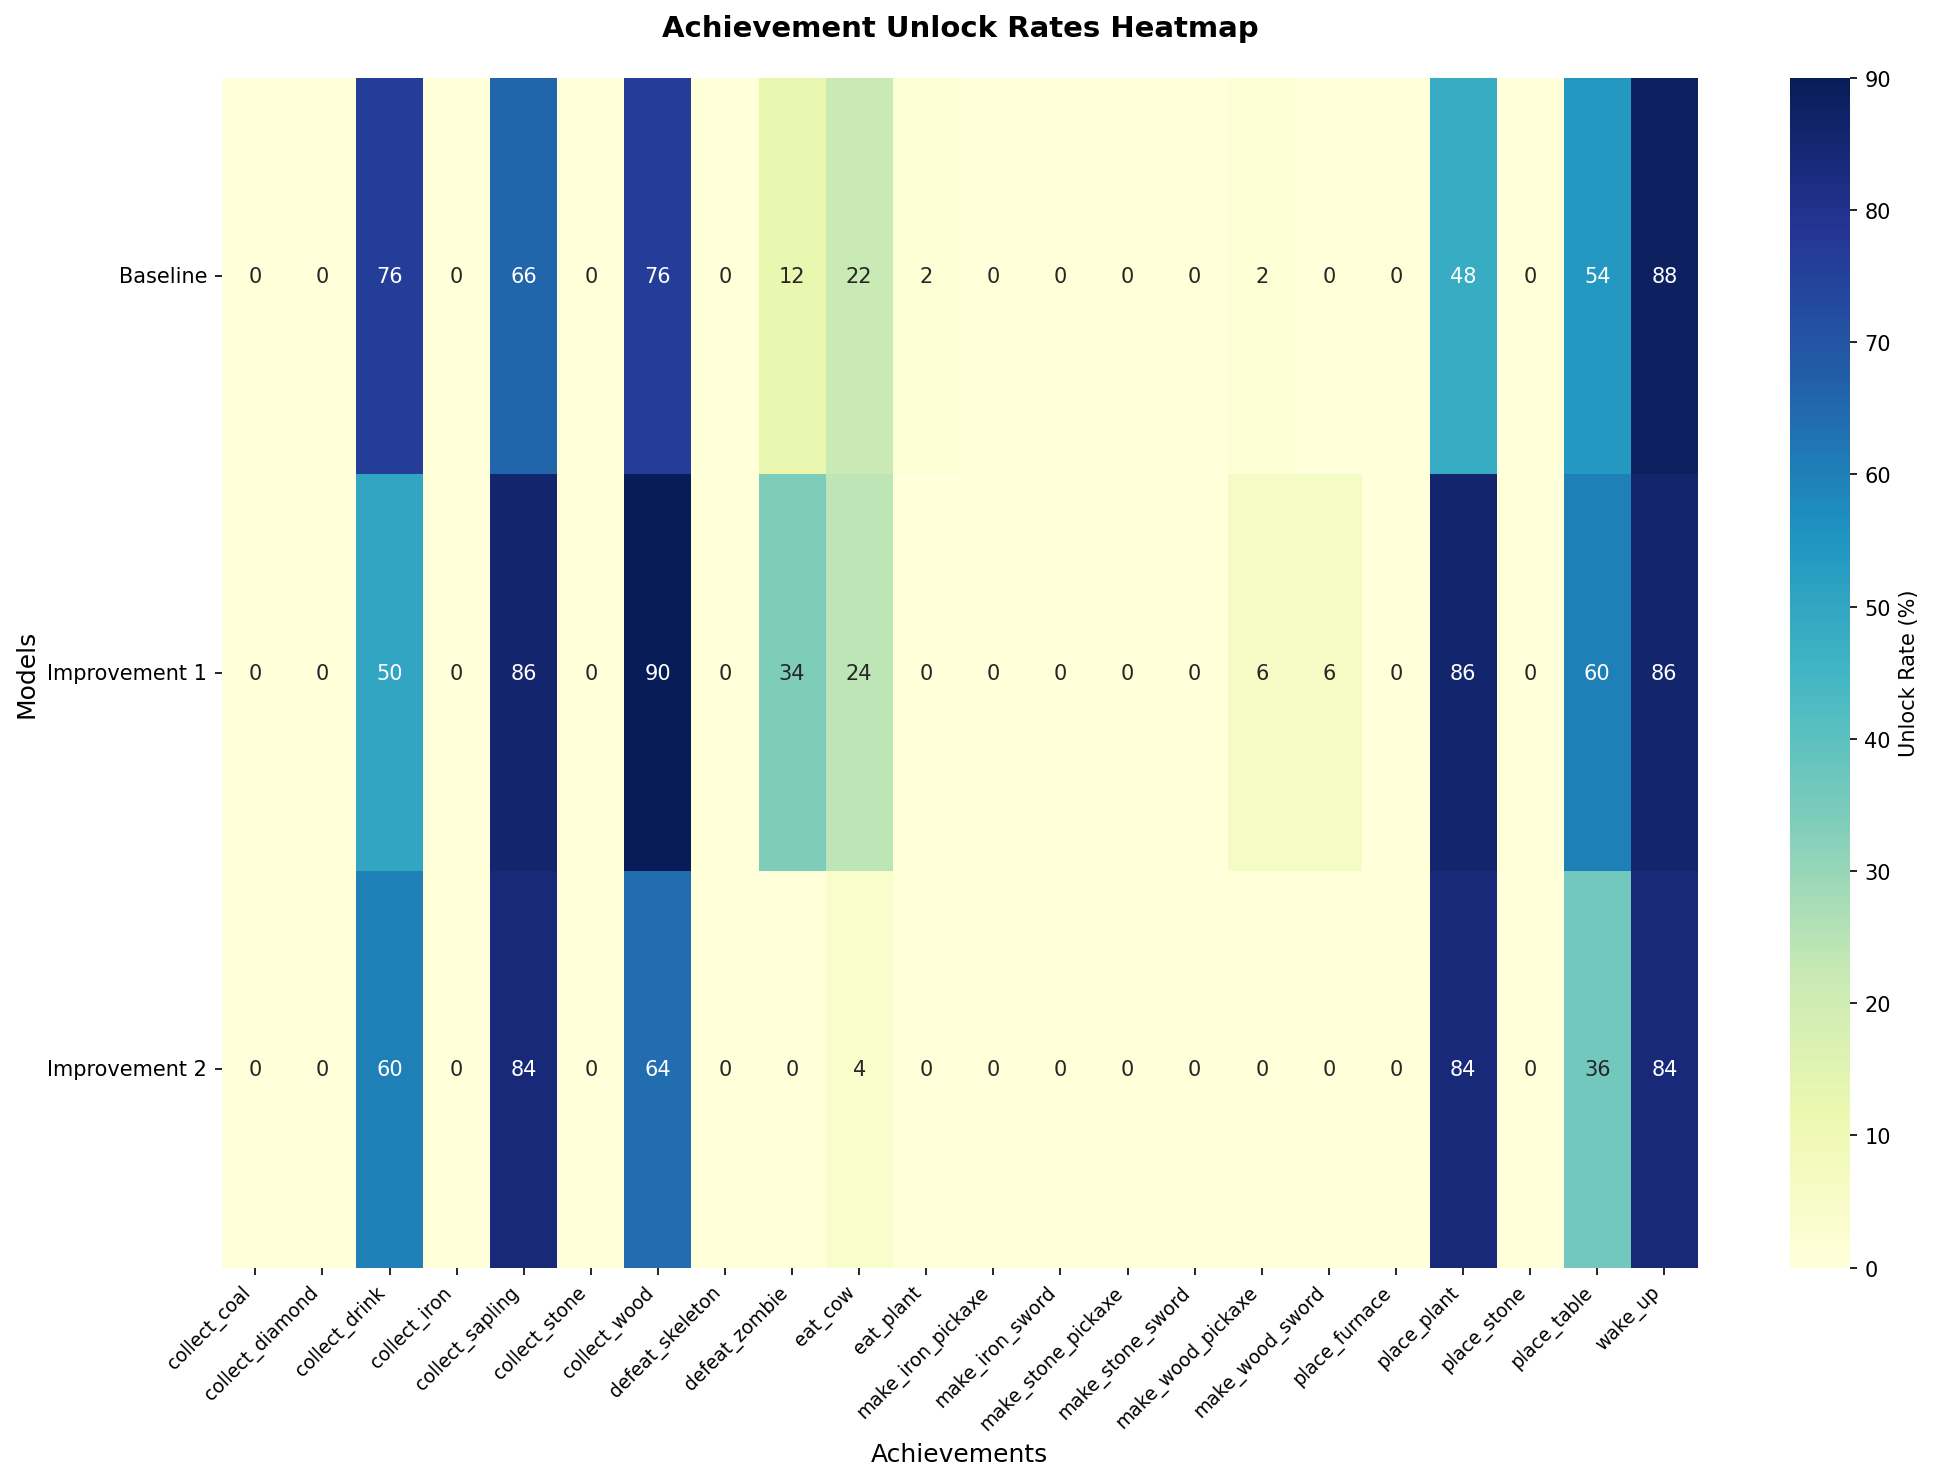
\includegraphics[width=0.8\linewidth]{images/DQNImprov2achievement_heatmap.png}
	\caption{A heatmap showing the achievements gained by each agent version.}
	\label{fig:dqn_comp_heatmap}
\end{figure}

\begin{itemize}
	\item \textbf{Mean reward:} Improvement 1 achieves a higher mean reward than Improvement 2, indicating more consistent policy performance in terms of immediate rewards.
	\item \textbf{Achievement progression:} Despite lower mean reward, Improvement 2 achieves a higher geometric mean and overall achievement performance, suggesting better multi-step planning and strategic progress.
	\item \textbf{Trade-off:} Improvement 1 favors short-term reward optimization, while Improvement 2 favors long-term achievement unlocking, highlighting the impact of residual CNN and frame-stacking in supporting temporal planning.
\end{itemize}

\section*{Out-of-class Algorithm: PPO}

PPO (Proximal Policy Optimization) is a reinforcement learning algorithm that trains an agent by optimizing its decision-making policy. It works by collecting data through interactions with an environment and then using a clipped objective function to make stable updates to the policy. This approach is known for being more stable, efficient, and easier to implement than some other policy gradient methods \parencite{schulman}.

\subsection*{Motivation}
PPO (Proximal Policy Optimization) is a good choice for the Crafter environment because it provides a strong balance of stability, sample efficiency, and simplicity while effectively handling the environment's key challenges, such as sparse rewards, long-term reasoning, and procedural generation. 

In addition these are the following theoretical benefits of PPO:
\begin{itemize}
    \item \textbf{Stable Policy Updates:} The Crafter environment is complex and dynamic, where large, unconstrained policy updates could easily destabilize training and cause the agent to forget beneficial behaviors. PPO's clipping mechanism limits how much the policy can change at each step, ensuring stable and controlled learning.
    \item \textbf{Sample Efficiency:} Crafter involves many different achievements and complex interactions, meaning efficient use of experience is crucial. PPO is relatively sample-efficient because it can reuse collected data over multiple training epochs (mini-batches) without significant instability, unlike other on-policy methods that only use data once.
    \item \textbf{Facilitates Exploration:} The PPO objective often includes an entropy bonus term, which encourages the agent to explore different actions and strategies. This is vital in Crafter, which features wide, procedurally generated worlds and independent achievements that require broad exploration to discover all possibilities.
\end{itemize}

\subsection*{Hyperparamters used across all agents}
\textbf{PPO Training:} These hyperparameters were standardized for all agents so as to make sure the comparison is done based on the differing algorithms and not hyperparameter tuning.
\begin{table}[H]
\centering
\caption{Hyperparameters used for PPO training}
\begin{tabular}{@{}ll@{}}
\toprule
\textbf{Hyperparameter} & \textbf{Value} \\ \midrule
Learning rate & $3 \times 10^{-4}$ \\
Rollout steps (\texttt{n\_steps}) & 2,048 \\
Batch size & 64 \\
Epochs per update & 10 \\
Discount factor ($\gamma$) & 0.99 \\
GAE lambda ($\lambda$) & 0.95 \\
Clip range & 0.2 \\
Entropy coefficient & 0.01 \\ \bottomrule
\end{tabular}
\end{table}

\subsection*{Baseline Implementation}
The baseline agent was implemented using the Stable-Baselines3 PPO algorithm. The initial hyperparameters were chosen to provide stable learning without aggressive updates, ensuring reproducibility. The agent at this point perceives the environment through single still images (frames) rather than continuous sequences, meaning it has only a limited view of the environment at each step.
\subsubsection*{Observations and Performance}
The baseline PPO agent exhibited some exploratory behavior and moderate learning progress. However, its limited temporal awareness significantly constrained performance. The average episodic reward stabilized around \textbf{2.66}, with the maximum reward achieved being \textbf{6.1}.
The following figures show the reward and survival distribution rates, as well as the achievement rates, over 1000 episodes:
\begin{figure}[H]
    \centering
    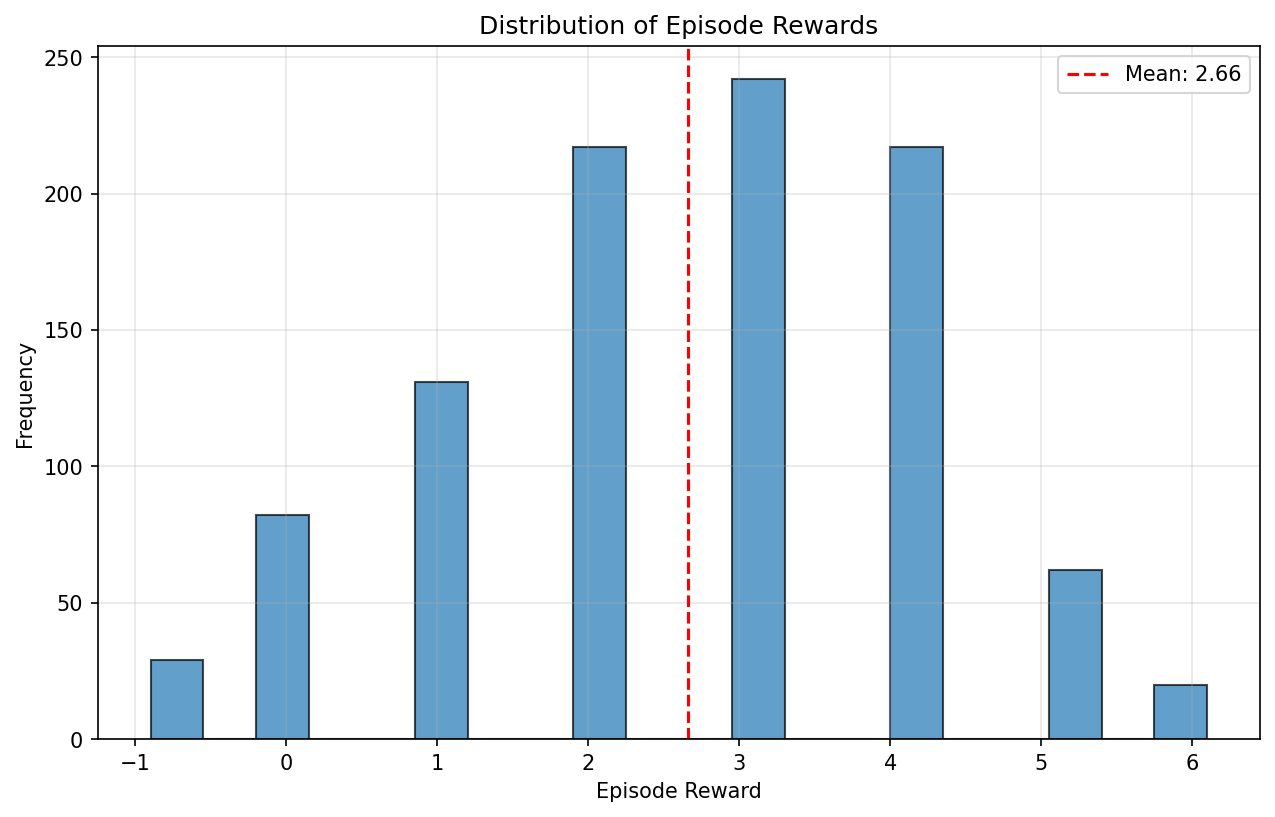
\includegraphics[width=0.75\linewidth]{images/reward_distribution_ppo_baseline_1000_episodes.png}
    \caption{Reward distribution of PPO baseline}
    \label{fig:placeholder}
\end{figure}
\begin{figure}[H]
    \centering
    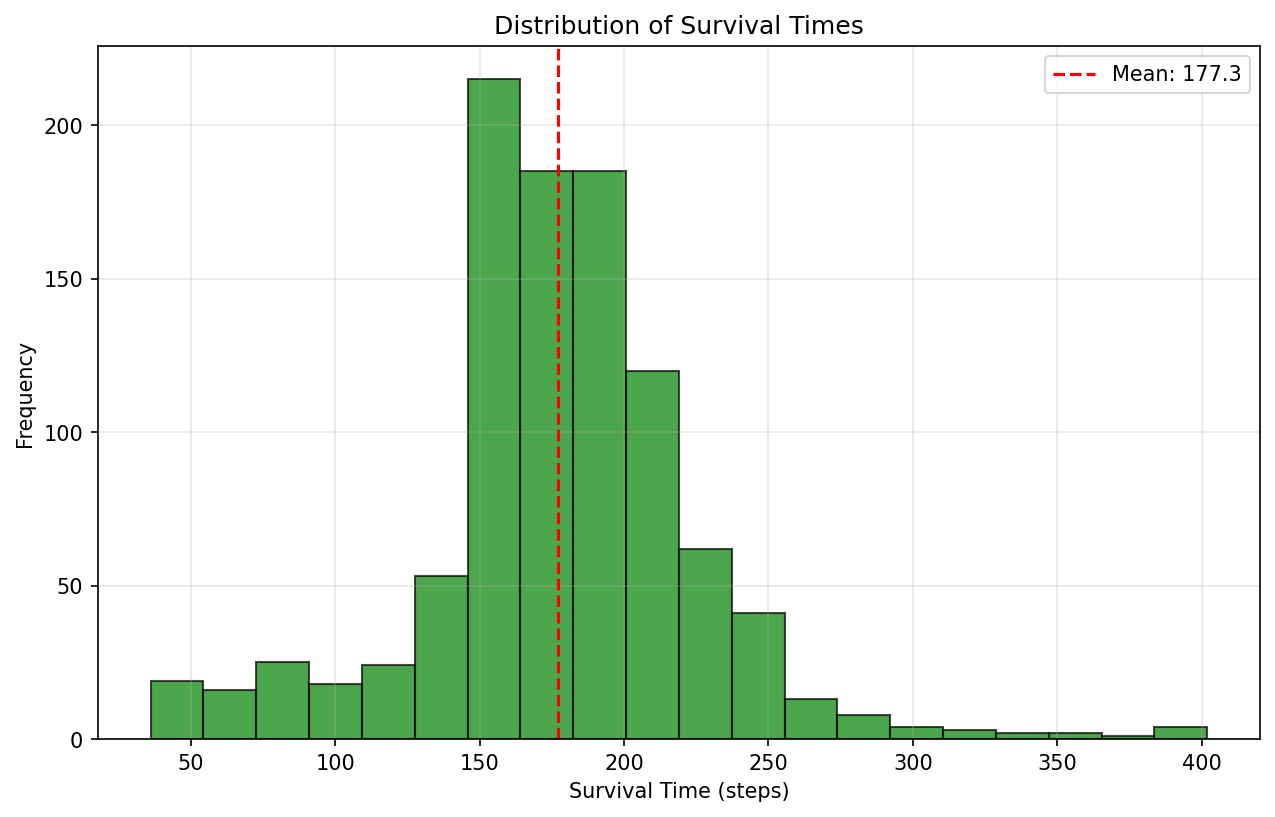
\includegraphics[width=0.75\linewidth]{images/survival_distribution_ppo_baseline_1000_episodes.png}
    \caption{Survival distribution of PPO baseline}
    \label{fig:placeholder}
\end{figure}
\begin{figure}[H]
    \centering
    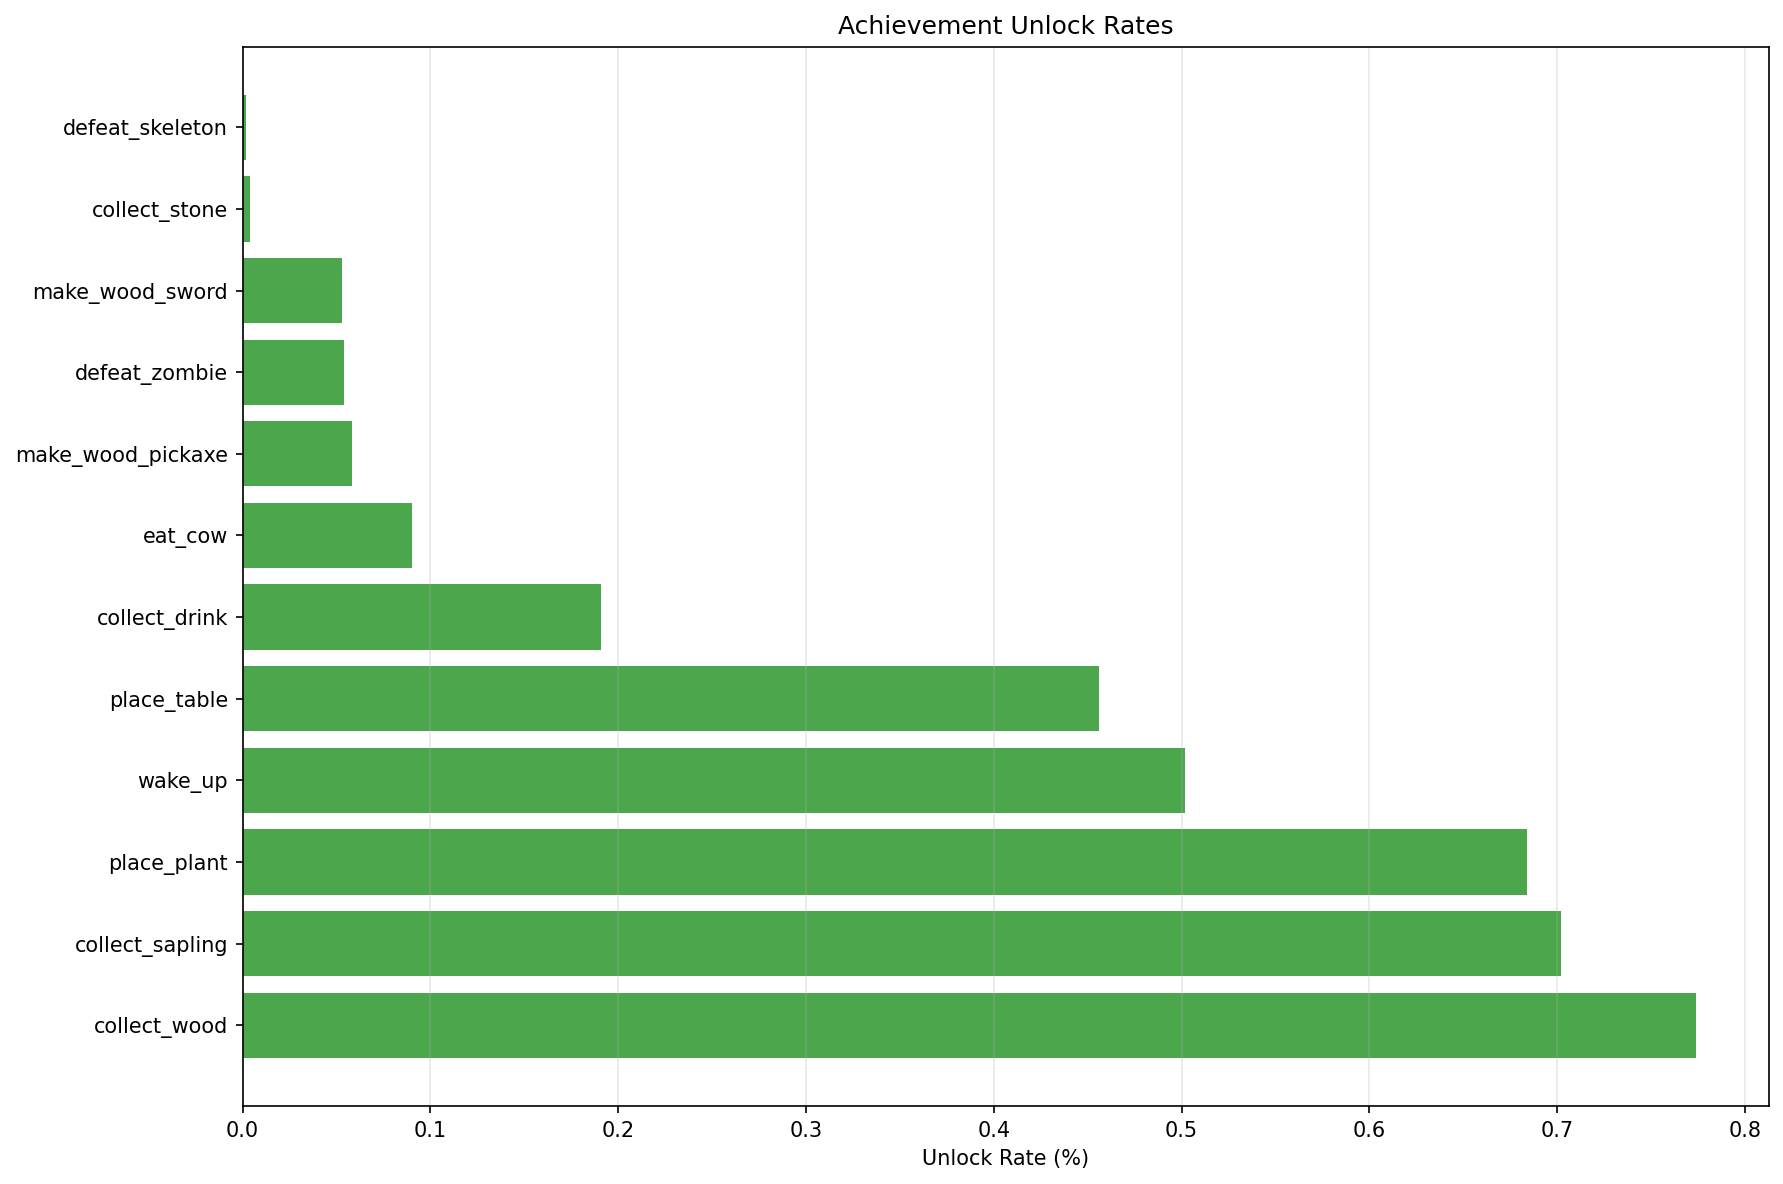
\includegraphics[width=0.75\linewidth]{images/achievement_rates_ppo_baseline_1000_episodes.png}
    \caption{Achievement rate of PPO baseline}
    \label{fig:placeholder}
\end{figure}
\subsubsection*{Identified areas of improvement}
The following weaknesses were identified in the baseline model:
\begin{itemize}
    \item \textbf{Lack of Memory:} The agent could recall previous states or actions, leading to suboptimal long-term decision-making.
    \item \textbf{Limited Exploration:} Without memory or intrinsic motivation, exploration remained shallow, resulting in repetitive behavior.
\end{itemize}


\subsection*{Improvement 1: Random Network Distillation}
\subsubsection*{Background}
Random Network Distillation (RND) is an exploration method that encourages reinforcement learning agents to explore novel states by providing intrinsic rewards based on prediction error. The method uses two neural networks: a target network that is randomly initialized and kept fixed, and a predictor network that is trained to predict the target network's outputs. The target network maps observations to feature vectors and remains frozen throughout training. The predictor network shares the same input-output architecture and is trained via gradient descent to minimize the mean squared error. The intrinsic reward is computed as the prediction error. This error is high for novel or infrequent states (where the predictor hasn't learned well) and low for frequently visited states (where the predictor has converged). \parencite{burda2018exploration}
\subsubsection*{Improvements}
RND is introduced to address the limited exploration of the baseline implementation. Because Crafter is an environment with sparce rewards, traditional reinforcement learning methods may not work as they rely on dense rewards. We hypothesise that RND should improve the average reward of the agent due in part to its larger exploration window, allowing for more opportunities for rewards to be obtained.

\subsubsection*{Methodology}
\textbf{\textit{Architecture}}\\
\textit{Target Network (Fixed Random Features)} \\
The target network is a randomly initialized convolutional neural network that remains fixed throughout training. It processes $64 \times 64 \times 3$ RGB observations through three convolutional layers:
\begin{itemize}
    \item Conv1: 32 filters, $3 \times 3$ kernel, stride 2, padding 1 $\rightarrow$ output: $32 \times 32 \times 32$
    \item Conv2: 64 filters, $3 \times 3$ kernel, stride 2, padding 1 $\rightarrow$ output: $16 \times 16 \times 64$
    \item Conv3: 64 filters, $3 \times 3$ kernel, stride 1, padding 1 $\rightarrow$ output: $16 \times 16 \times 64$
    \item Flatten and fully connected layers: $16{,}384 \rightarrow 512$ features
\end{itemize}

All parameters are frozen after initialization to maintain consistent random target features.\\\\
\textit{Predictor Network (Learned Features)} \\
The predictor network shares an identical architecture with the target network but is trained to predict the target network's output. The prediction error serves as the intrinsic reward signal, where high error indicates novel states.\\\\
\textbf{\textit{Intrinsic Reward Computation}}\\
For each observed state $s_t$, the intrinsic reward is computed as:
\begin{equation}
r_{\text{intrinsic}}(s_t) = \|f_{\text{target}}(s_t) - f_{\text{predictor}}(s_t)\|^2
\end{equation}
where $f_{\text{target}}$ and $f_{\text{predictor}}$ are the outputs of the target and predictor networks respectively. The intrinsic rewards are normalized using running mean and variance statistics to maintain stable learning dynamics.\\\\
\textbf{\textit{Reward Integration}}\\
The total reward combines extrinsic (environment) and intrinsic rewards:
\begin{equation}
r_{\text{total}}(s_t) = r_{\text{extrinsic}}(s_t) + \lambda \cdot r_{\text{intrinsic}}(s_t)
\end{equation}
where $\lambda$ is the intrinsic reward coefficient (set to 1.0 by default). This is implemented via a custom Gymnasium wrapper (\texttt{RNDRewardWrapper}) that intercepts environment steps and augments rewards before they reach the PPO algorithm.\\\\
\textbf{\textit{Training Procedure}}
\begin{itemize}
    \item \textbf{RND Module Updates:} The predictor network is trained using mean squared error loss between its outputs and the fixed target network outputs. The optimizer uses Adam with learning rate $1 \times 10^{-4}$.

    \item \textbf{PPO Training:} The PPO agent is trained over $3\times10^6$ timesteps on the combined reward signal using standard hyperparameters and the following:
\begin{itemize}
    \item $intrinsic\_reward\_coef=1.0$
    \item $rnd\_learning\_rate=1\times10^{-4}$
\end{itemize}

\item \textbf{Evaluation Protocol:} Agent performance is evaluated every 10,000 training steps using deterministic policy rollouts over 5 episodes in a separate evaluation environment. Metrics including mean reward, standard deviation, minimum/maximum rewards, and episode lengths are logged to CSV files for analysis.
\end{itemize}
\textbf{\textit{Exploration Mechanism}}\\
The RND method encourages exploration through the following mechanism:
\begin{enumerate}
    \item Novel states produce high prediction errors, yielding high intrinsic rewards
    \item The agent is incentivized to visit these high-reward states
    \item As states become familiar, the predictor improves, reducing intrinsic rewards
    \item The agent naturally shifts focus toward extrinsic task rewards
\end{enumerate}
This approach addresses the sparse reward problem in Crafter by providing dense exploration bonuses while maintaining the original task structure.\\\\
\textbf{\textit{Implementation Details}}\\
The implementation utilizes PyTorch for neural networks and Stable Baselines3 for the PPO algorithm. The RND networks use $3 \times 3$ convolutional kernels optimized for Crafter's $64 \times 64$ observation space. Running statistics for reward normalization use Welford's online algorithm to maintain numerical stability. All experiments use seed 42 for reproducibility, with the evaluation environment seeded at 142 to ensure different but deterministic trajectories.
\subsubsection*{Results}
The agent was evaluated over 1000 episodes, giving an average reward of \textbf{3.3} and a maximum reward of \textbf{7.1}. This is an improvement of around \textbf{24\%} and around \textbf{16\%} over the average reward and maximum reward, respectively. This provides evidence that with RND, the average reward obtained improves from the baseline. However, this is a minor improvement and further improvements can be made by tuning the hyperparameters of the RND networks or running the training for more timesteps, which may give the agent more opportunities to explore novel states. Below are the figures showing the reward and survival distribution rates, as well as the achievement rates, over 1000 episodes:
\begin{figure}[H]
    \centering
    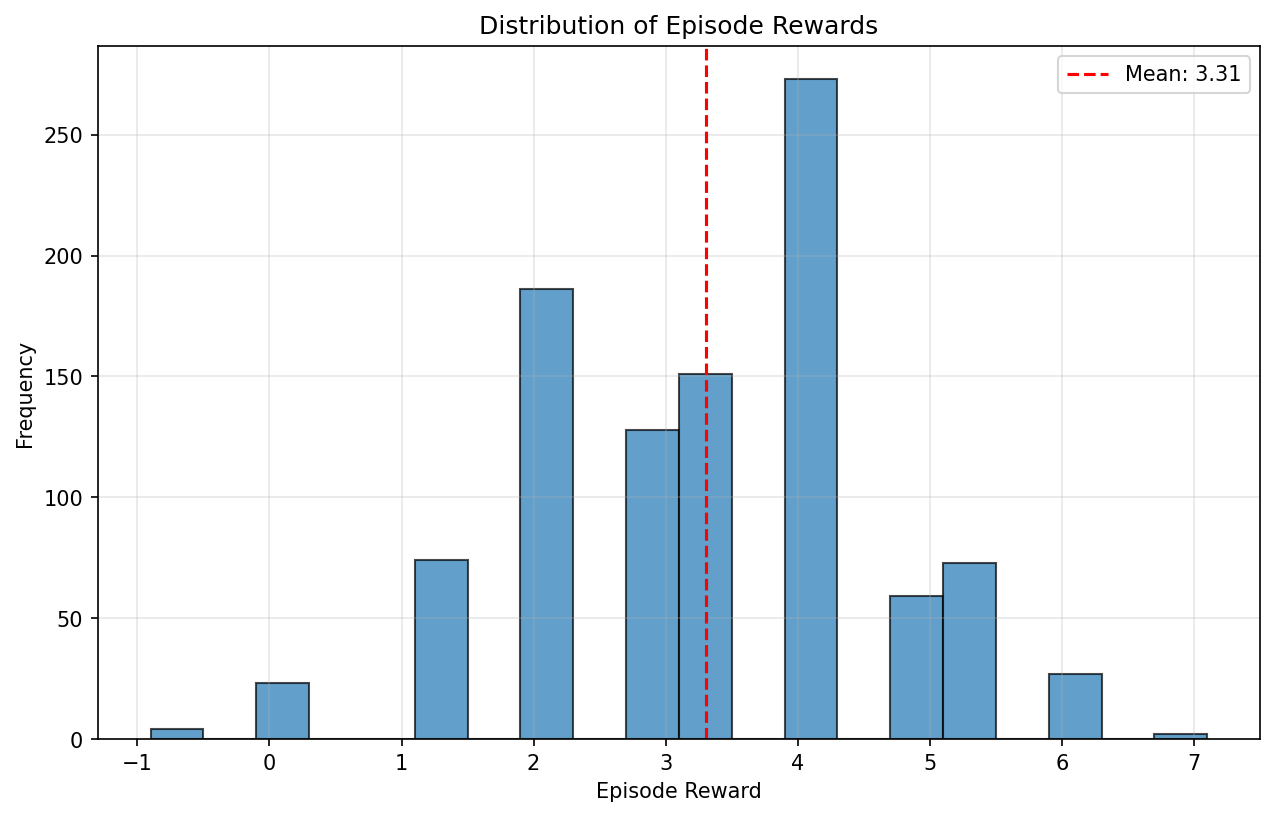
\includegraphics[width=0.75\linewidth]{images/reward_distribution_ppo_improv1_1000_episodes.png}
    \caption{Reward distribution of PPO-RND}
    \label{fig:placeholder}
\end{figure}
From this figure, the RND agent receives higher rewards more frequently than the baseline. This makes sense since by trying novel actions, there are more possibilities for rewards. However, a consequence of this is that the frequency of different rewards is not as uniform as the baseline.
\begin{figure}[H]
    \centering
    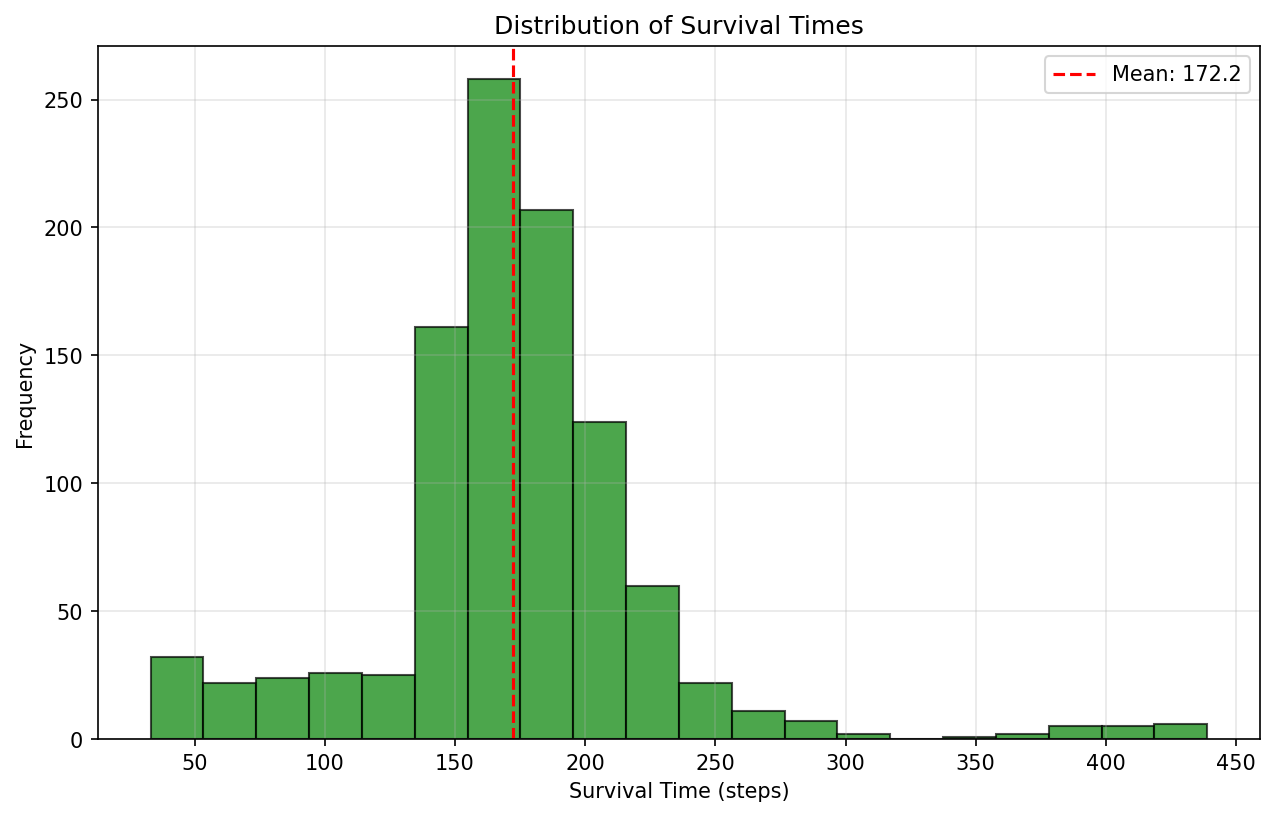
\includegraphics[width=0.75\linewidth]{images/survival_distribution_ppo_improv1_1000_episodes.png}
    \caption{Survival distribution of PPO baseline}
    \label{fig:placeholder}
\end{figure}
The RND figure in comparison to the baseline shows that the baseline tends to survive longer than the improvement. This can also be explained by the fact that the agent is more likely to explore - through more exploration comes more opportunities to enter states that lead the agent to die.
\begin{figure}[H]
    \centering
    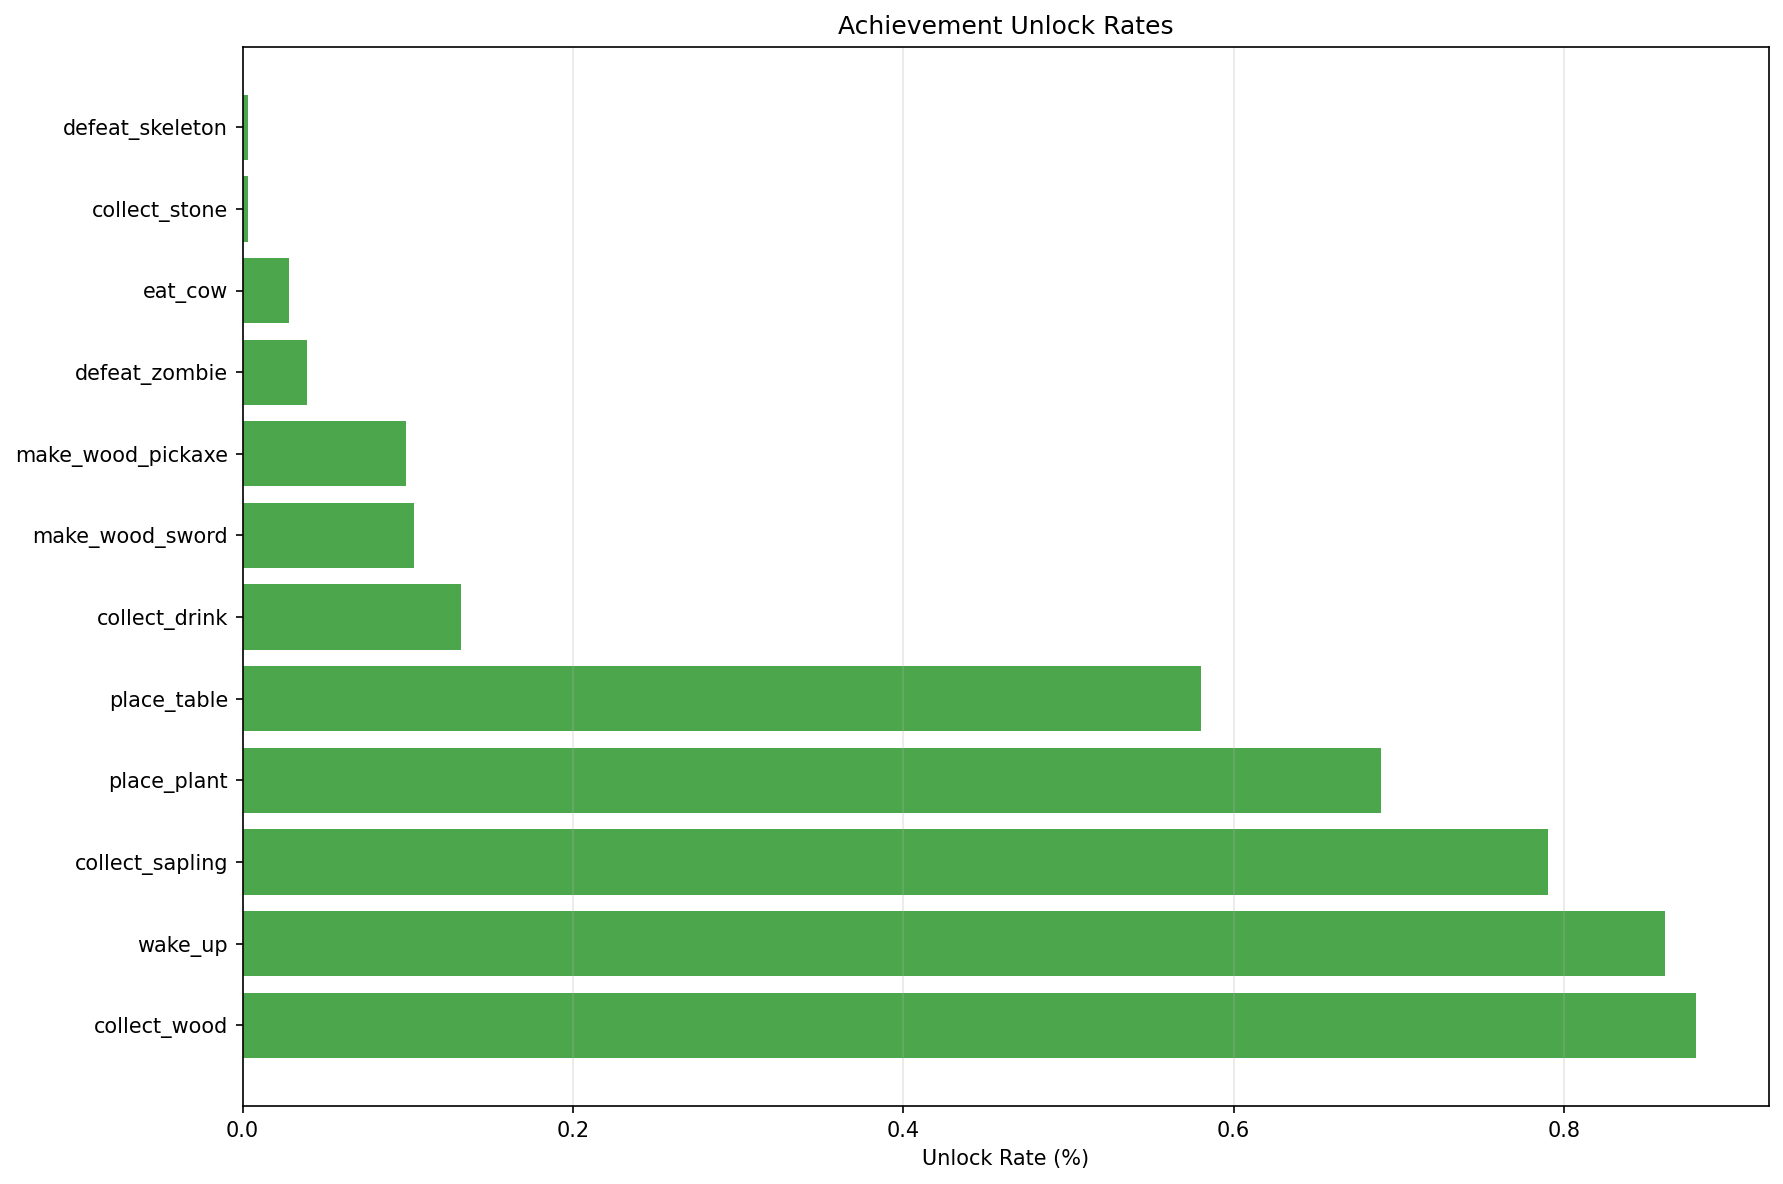
\includegraphics[width=0.75\linewidth]{images/achievement_rates_ppo_improv1_1000_episodes.png}
    \caption{Achievement rate of PPO baseline}
    \label{fig:placeholder}
\end{figure}
This figure shows that, in comparison to the baseline, the RND agent will have a less consistent spread of acheivement unlock rates since the agent is encouraged to choose novel states. While the baseline shows that over time the agent learns to repeat tasks that will provide it more rewards in the future, the RND has high achievement rates on tasks that won't offer much benefit to the agent, such as placing plants, or not eating and drinking as much.
\subsubsection*{Discussion}
\textbf{\textit{Strengths and weaknesses}}\\
The strengths of this implementation follow as a consequence of its approach. Because the agent is encouraged to explore more, the agent is more likely to unlock more acheivements, receive greater rewards, and learn more aboout the environment at a faster rate as compared to the baseline. However, its weaknesses are that it requires far more training time than the baseline since there is a large number of possible states to explore and similar to Monte Carlo exploration, requires a large numebr of episodes to get a good idea of the environment and its dynamics. Another weakness of the current RND implementation is the context window is very small, and thus even when the agent unlocks new achievements, these achievements and the rewards associated with them aren't carrying over in future.\\
\textbf{\textit{Differences from Standard RND Implementation}}\\
This implementation differs from the standard Random Network Distillation approach proposed by \cite{burda2018exploration} in several key aspects. The standard RND implementation uses two separate value functions---one for extrinsic returns and one for intrinsic returns---allowing different discount factors to be applied (typically $\gamma=0.99$ for intrinsic and $\gamma=0.999$ for extrinsic rewards), whereas this implementation uses a single combined value function with a uniform discount factor of 0.99. The CNN architecture has been simplified and adapted for Crafter's $64 \times 64$ observation space, using smaller $3 \times 3$ kernels throughout instead of the larger $8 \times 8$ and $4 \times 4$ kernels designed for $84 \times 84$ Atari frames, and omitting batch normalization and other regularization layers. Unlike standard RND which normalizes observations before feeding them to the RND networks and maintains separate statistics for intrinsic and extrinsic rewards, this implementation applies only basic running statistics normalization to intrinsic rewards using Welford's algorithm, with raw observations fed directly to the networks. The standard approach typically employs 128 or more parallel environments for efficient data collection and diverse training batches, updating the predictor network on mini-batches from the rollout buffer with multiple gradient steps per rollout, whereas this implementation uses a single environment instance with per-step predictor updates, resulting in slower data collection and potentially noisier gradient estimates. Additionally, standard RND implementations include explicit reward clipping to prevent extreme values, separate advantage normalization for intrinsic and extrinsic components, and curiosity-driven exploration decay schedules, none of which are present in this implementation which uses a fixed intrinsic reward coefficient. Finally, the evaluation procedure differs: standard RND evaluates with intrinsic rewards completely disabled to measure true task performance without exploration bonuses, while this implementation uses deterministic policy evaluation without explicitly disabling the RND wrapper, making the separation between exploration and exploitation performance less clear.
\subsection*{Improvement 2: Long-Short Term Memory}

\subsubsection*{Background}

RecurrentPPO is an extension of the Proximal Policy Optimization (PPO) algorithm that adds support for recurrent neural network policies, specifically using LSTM (Long Short-Term Memory) layers. This implementation allows the agent to maintain memory of past observations and actions, making it particularly useful for partially observable environments where the full state isn't available at each timestep \parencite{salim}.

\subsubsection*{Improvements}
To address the baseline and improvement 1 limitations in memory and exploration, we implemented a \textbf{Recurrent Proximal Policy Optimization (Recurrent PPO)} agent. The memory mechanism helps the agent handle the partially observable nature of the Crafter environment, where important state information may not be visible in a single frame.

The following hyperparameters were added in addition to the previous implementations:

\begin{itemize}
    \item \textbf{Value function coefficient ($vf\_coef$):} 0.5
    \item \textbf{Max. gradient norm ($max\_grad\_norm$):} 0.5
\end{itemize}

Moreover, slight reward shaping was employed to accelerate convergence and guide exploration towards useful sub-goals. This ensured that intermediate achievements (such as crafting tools or collecting resources) contributed meaningful gradient signals during training.
\subsubsection*{Methodology}

This implementation employs \textbf{RecurrentPPO with a MultiInputLstmPolicy architecture} applied to the Crafter environment, using standard hyperparameters.

A few \textbf{domain-specific enhancements} distinguish this implementation from basic RecurrentPPO. First, a multi-modal observation space architecture combines image observations with a discrete 22-dimensional achievement vector tracking task completion states such as resource collection, crafting milestones, and survival events. This dual-stream observation design allows the LSTM to learn both spatial-temporal patterns from visual data and discrete progress indicators simultaneously.

Second, the implementation incorporates \textbf{intrinsic reward shaping} through three components: achievement bonuses (5.0\(\times\) multiplier for newly completed achievements), survival bonuses (+0.01 per timestep), and exploration bonuses (+0.001 per action). This additional reward signal addresses sparse reward problems inherent to open-ended exploration tasks, encouraging the agent to try different behaviors beyond the base environment rewards.

\subsubsection*{Results}
The introduction of temporal recurrence through an LSTM notably improved the agent's ability to integrate information across time steps. Compared to the baseline PPO model, which achieved a mean episodic reward of approximately 2.66 (maximum 6.1), the Recurrent PPO (R-PPO) demonstrated consistent performance gains achieving a mean episodic reward of 4.71 (maximum 11.1) as viewed in the figure below: 
\begin{figure}[H]
    \centering
    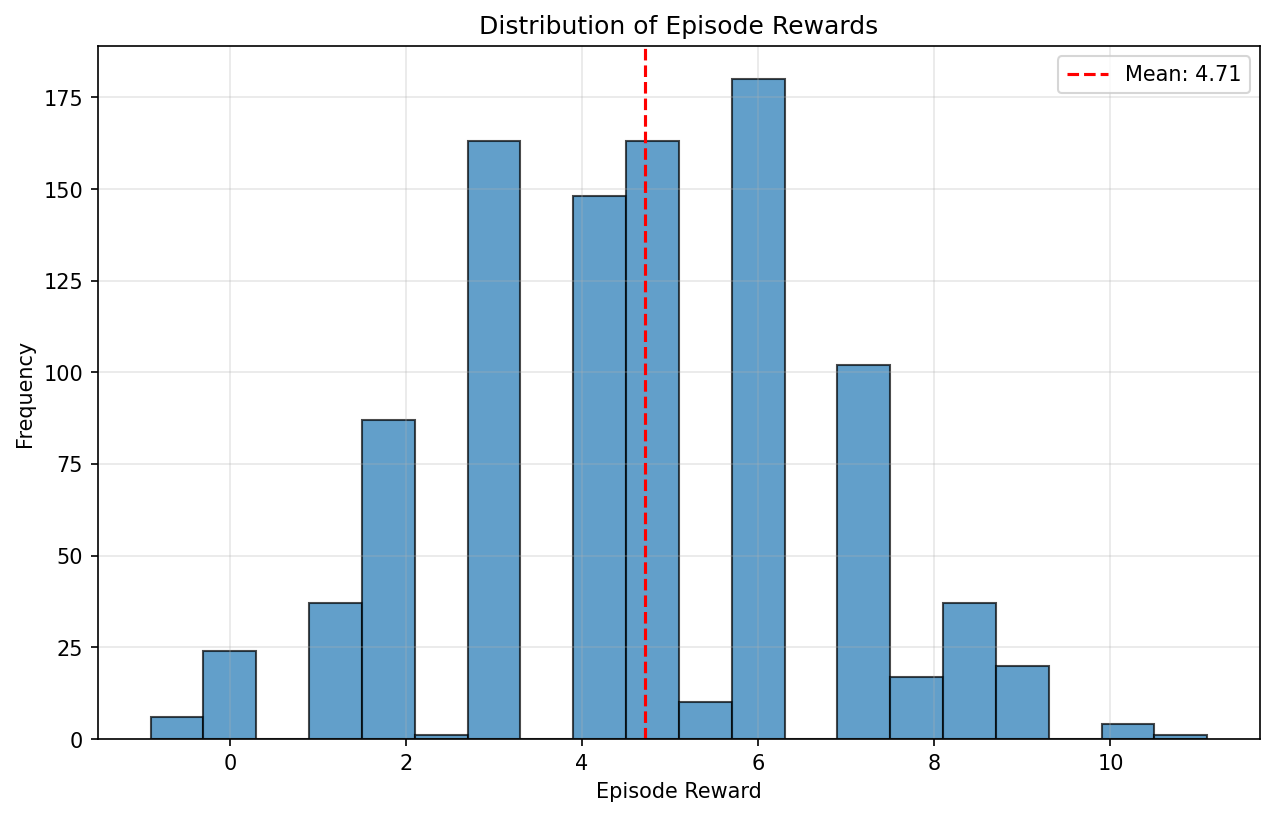
\includegraphics[width=0.75\linewidth]{images/reward_distribution_ppo_improv2_1000_episodes.png}
    \caption{Reward distribution of RecurrentPPO}
    \label{fig:placeholder}
\end{figure}

\subsubsection*{Qualitative Observations}

Behaviorally, the Recurrent PPO agent demonstrated:
\begin{itemize}
    \item More coherent decision sequences across time, owing to the LSTM's memory retention.
    \item Improved persistence in long-horizon tasks such as crafting and navigation.
    \item Less tendency to repeat suboptimal exploration patterns seen in the baseline agent.
\end{itemize}

In addition, reward shaping contributed to smoother early learning and faster convergence during training, as the agent received structured feedback for intermediate achievements.

\subsubsection*{Discussion}

The performance gain from incorporating temporal memory validates the hypothesis that Crafter's partial observability penalizes stateless architectures. By maintaining a hidden state, the Recurrent PPO agent effectively constructs an implicit representation of unobserved parts of the environment. This allows for more context-aware actions and ultimately leads to higher cumulative rewards. 

While the improvement is evident, the results also reveal that the agent has not fully stabilized, indicated by the wide reward range. Further tuning of learning rate, clipping threshold, and recurrent hidden size could reduce variance and enhance consistency across episodes.

The following figures show the different achievement and survival distribution rates over 1000 episodes:
\begin{figure}[H]
    \centering
    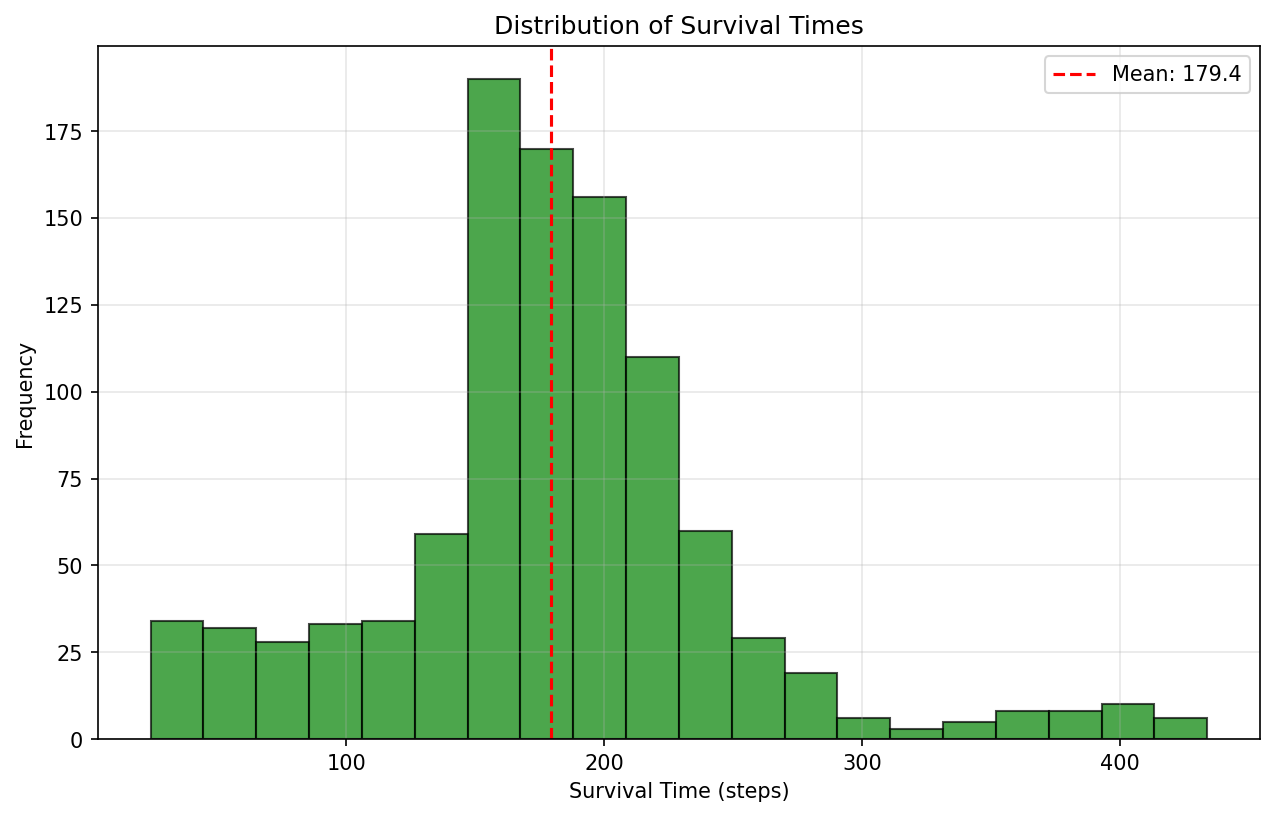
\includegraphics[width=0.75\linewidth]{images/survival_distribution_ppo_improv2_1000_episodes.png}
    \caption{R-PPO Survival Distribution rate}
    \label{fig:placeholder}
\end{figure}

\begin{figure}[H]
    \centering
    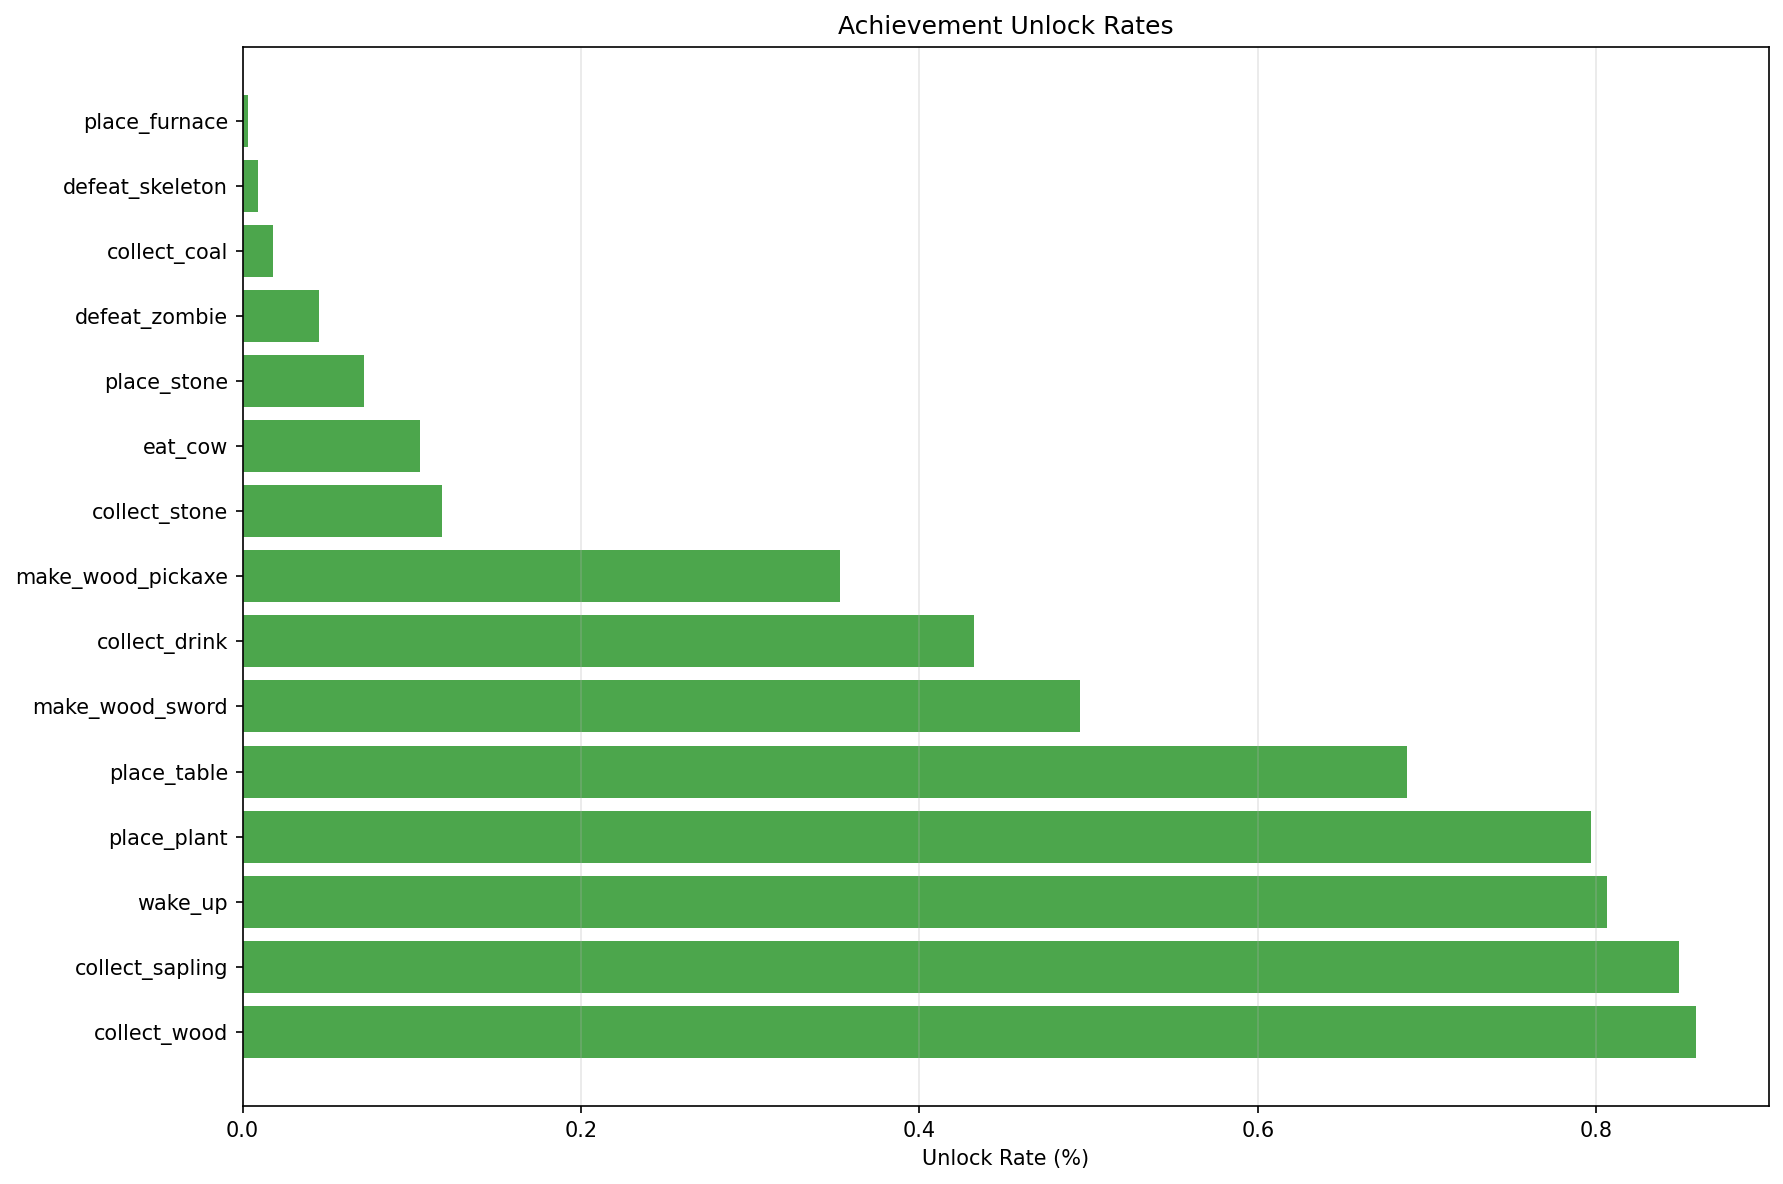
\includegraphics[width=0.75\linewidth]{images/achievement_rates_ppo_improv2_1000_episodes.png}
    \caption{R-PPO Achievement Distribution rate}
    \label{fig:placeholder}
\end{figure}


An interesting observation from the experiments was that the Recurrent PPO  agent achieved a higher average reward (4.71) than the baseline PPO (2.66), despite exhibiting a lower overall survival rate. This contradiction can be explained by the agent's behavioral bias toward short-term, high-value actions.

The inclusion of memory through the LSTM layer allowed the agent to recall and exploit previously observed opportunities, such as nearby resources or enemies, resulting in higher reward density per timestep. However, this same decisiveness increased exposure to risk, reducing overall survival time.

Additionally, the use of reward shaping likely amplified this effect by reinforcing immediate sub-goal completion (e.g., crafting, combat) rather than conservative, long-term survival strategies. Consequently, the R-PPO learned to act more efficiently but less cautiously, prioritizing cumulative reward over lifespan duration.

This highlights a fundamental reinforcement learning trade-off between \textit{reward maximization} and \textit{survival optimization}, emphasizing that longer episodes do not necessarily equate to better task performance.

\section*{PPO Consolidation}
\begin{figure}[H]
    \centering
    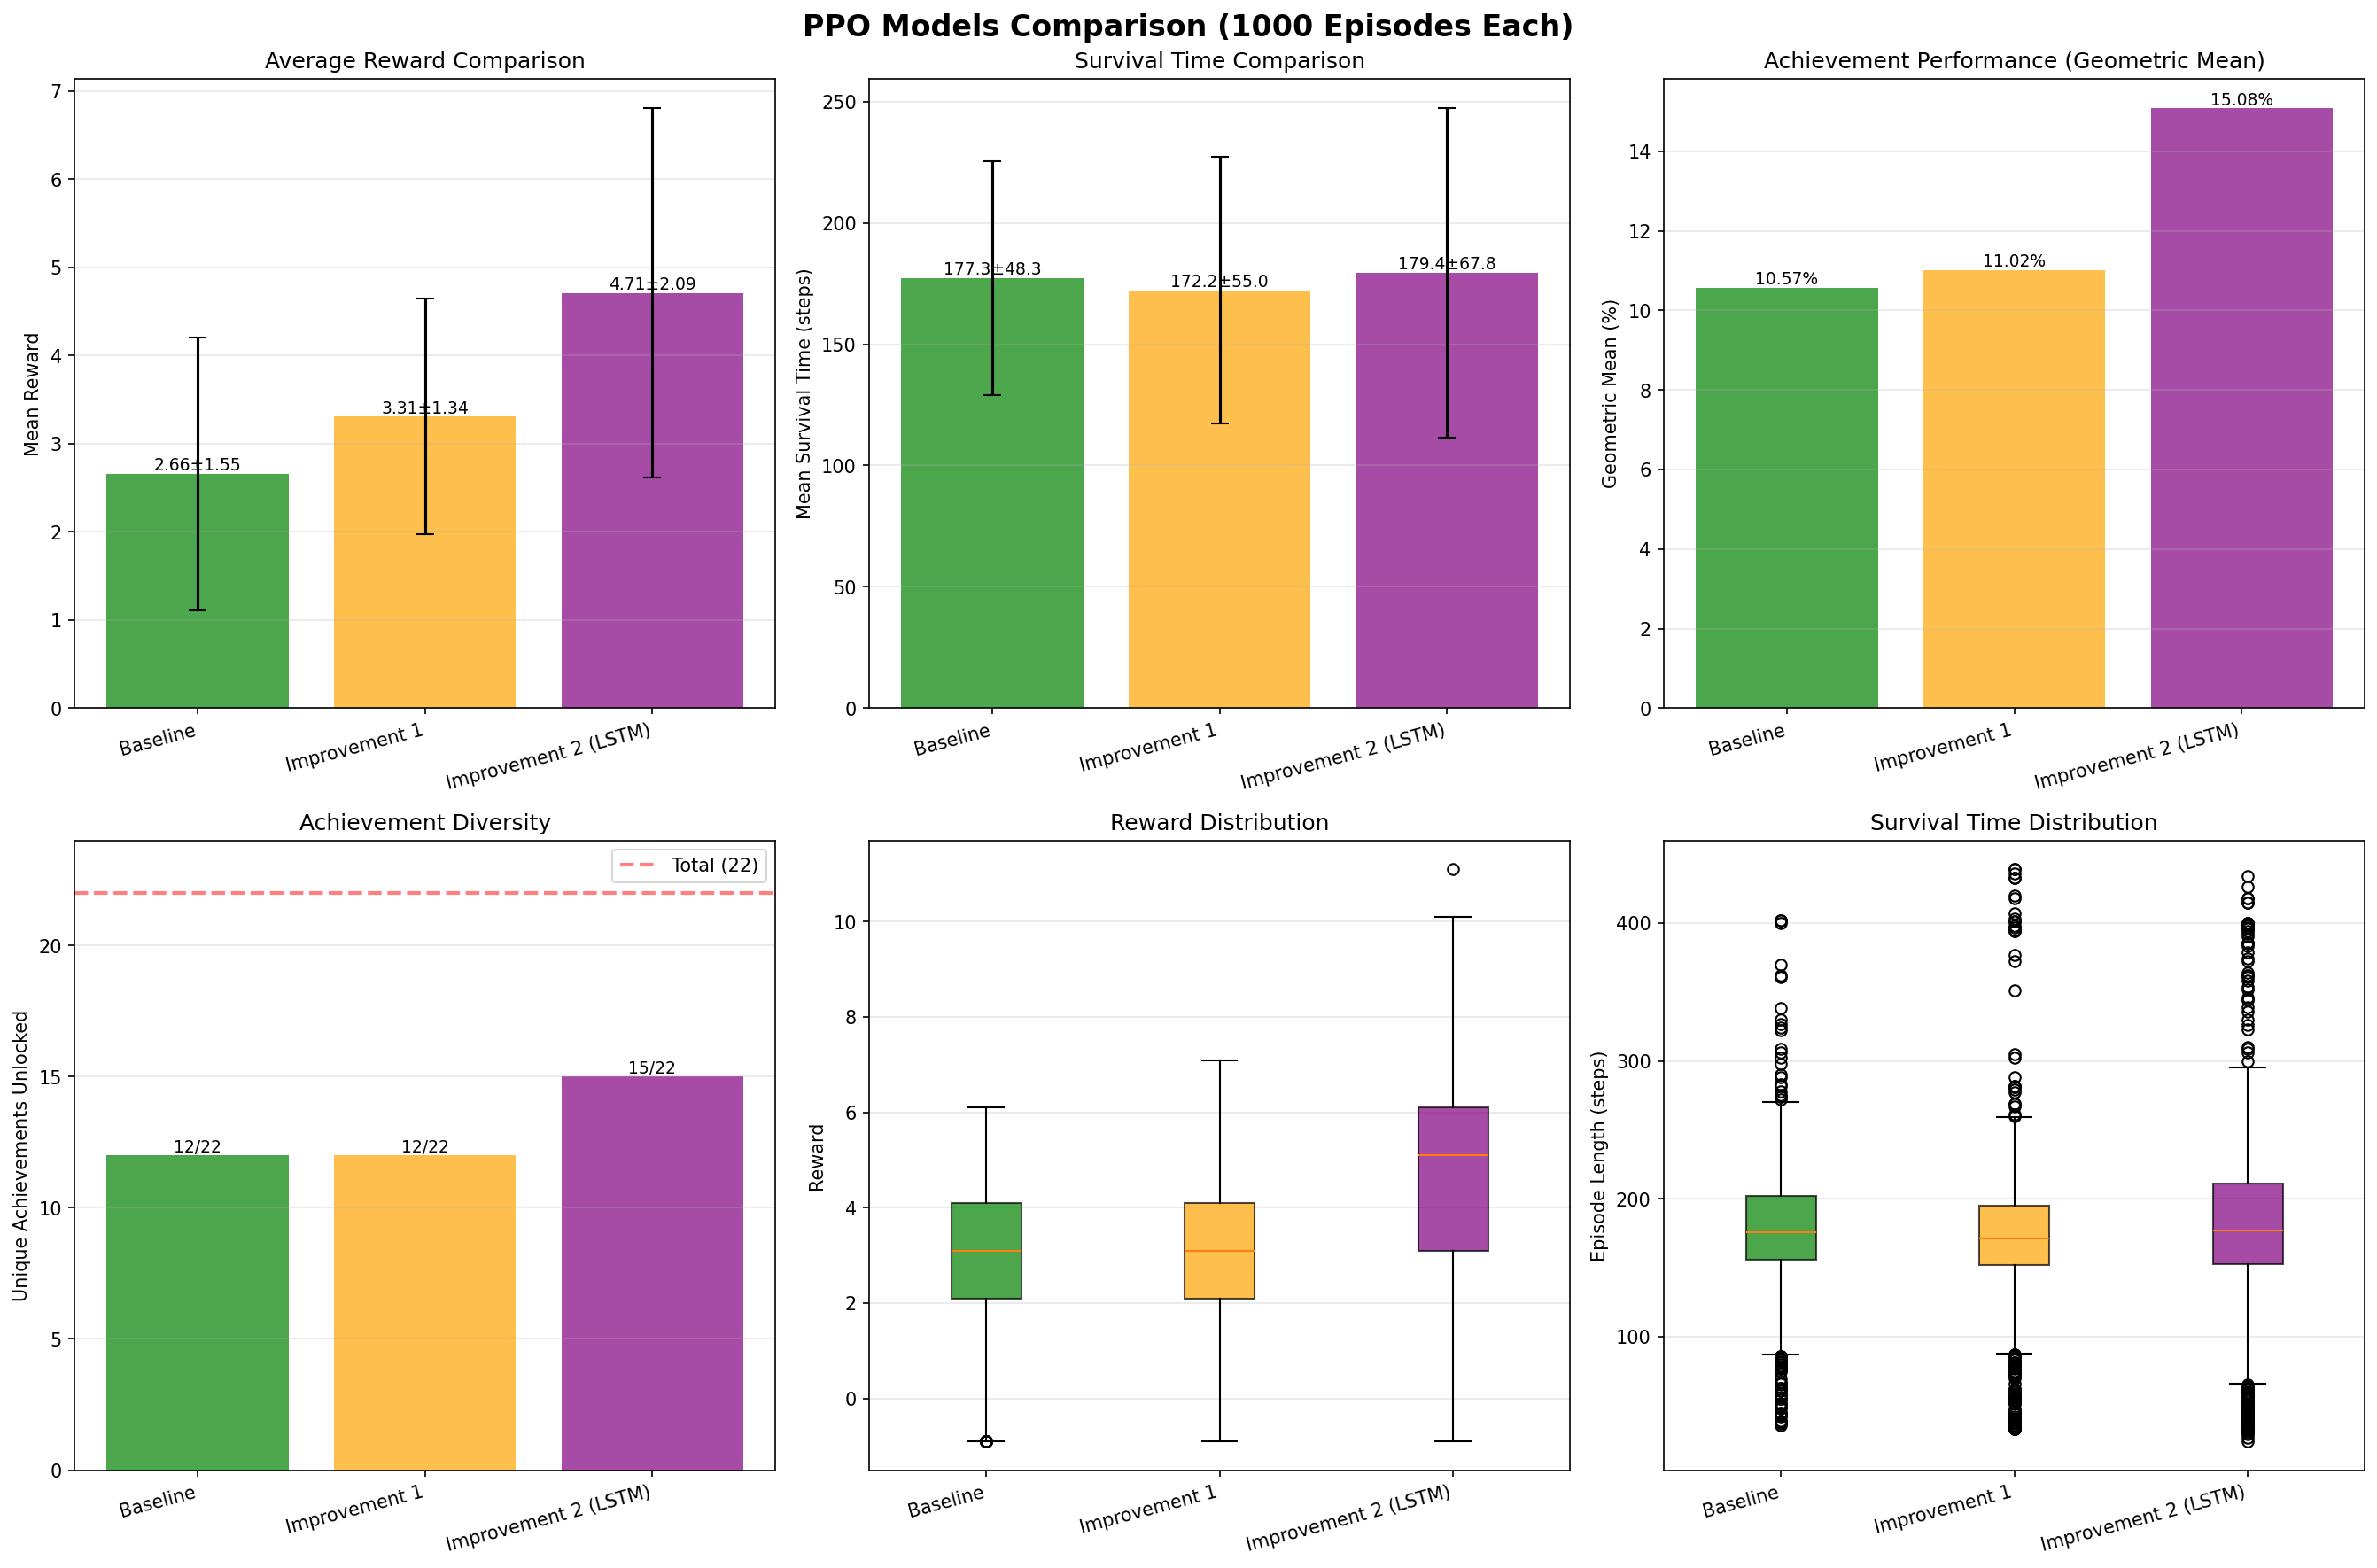
\includegraphics[width=0.75\linewidth]{images/final_comparison_1000_episodes.png}
    \caption{All PPO algorithms compared across metrics.}
    \label{fig:placeholder}
\end{figure}

\section*{DQN vs PPO}
\section*{Conclusion}
\printbibliography

\end{document}
